\documentclass[12pt,a4paper,titlepage,listof=totoc,bibliography=totoc,chapteratlists=0pt]{scrreprt}

\begin{filecontents*}{\jobname.xmpdata}
	\Keywords{IOT}
	\Title{APERTA}
	\Author{Benjamin Golic, David Hauser, Simon Koll}
\end{filecontents*}

\setcounter{tocdepth}{1}

\usepackage[utf8]{inputenc}
\usepackage[T1]{fontenc}
\usepackage{amsmath}
\usepackage{amsfonts}
\usepackage{amssymb}
\usepackage[table]{xcolor}
\usepackage{graphicx}
\usepackage[left=3.50cm, right=2.00cm, top=2.00cm, bottom=2.00cm,foot=1cm]{geometry}
\usepackage[splitrule,hang,flushmargin,multiple,bottom]{footmisc}
\usepackage{lmodern, textcomp}
\usepackage{lmodern}
\usepackage{pdfpages}
\usepackage[ngerman]{babel}
\usepackage{multicol}
\usepackage{subfig}
\usepackage{float}
\usepackage{array,tabularx,booktabs}
\usepackage{ragged2e}
\usepackage{lipsum}
\usepackage{wrapfig}
\usepackage{svg}
\usepackage{amsmath}
\usepackage{booktabs}
\usepackage{adjustbox,lipsum}
\usepackage{subfig}
\usepackage{xcolor}

\newcolumntype{M}[1]{>{\centering\arraybackslash}m{#1}}

\usepackage{enumitem}
\newlist{compactitem}{itemize}{3}
\setlist[compactitem,1]{label=\textbullet, nosep,leftmargin=1.5em,labelwidth=*,align=left}
\setlist[compactitem,2]{label=--, nosep,leftmargin=1.5em,labelwidth=*,align=left}
\setlist[compactitem,3]{label=\textopenbullet, nosep,leftmargin=1.5em,labelwidth=*,align=left}
\newlist{compactenum}{enumerate}{3}
\setlist[compactenum,1]{label=\arabic*., nosep,leftmargin=1.5em,labelwidth=*,align=left}
\setlist[compactenum,2]{label=\alph*., nosep,leftmargin=1.5em,labelwidth=*,align=left}
\setlist[compactenum,3]{label=\roman*., nosep,leftmargin=1.5em,labelwidth=*,align=left}
\newlist{compactdesc}{description}{3}
\setlist[compactdesc]{leftmargin=1.5em,labelwidth=*,align=left}

\usepackage{microtype}

\usepackage[parfill]{parskip}

\definecolor{bluekeywords}{rgb}{0.13,0.13,1}
\definecolor{greencomments}{rgb}{0,0.5,0}
\definecolor{redstrings}{rgb}{0.9,0,0}
\definecolor{lightgray}{gray}{0.9}
\definecolor{lightblue}{rgb}{0.93,0.95,1.0}
\definecolor{mygreen}{rgb}{0,0.6,0}
\definecolor{mygray}{rgb}{0.5,0.5,0.5}
\definecolor{mymauve}{rgb}{0.58,0,0.82}
\definecolor{darkgray}{rgb}{.4,.4,.4}
\definecolor{purple}{rgb}{0.65, 0.12, 0.82}


\usepackage{listings}

\makeatletter
\lstdefinestyle{lststyle}{
	basicstyle=%
	\ttfamily
	\lst@ifdisplaystyle\scriptsize\fi
}
\makeatother

\renewcommand{\lstlistlistingname}{List of Listings}
% TODO: define other languages as needed
\lstset{language=Python,
numbers=left,               
numberstyle=\tiny,          
showspaces=false,
showtabs=false,
breaklines=true,
lineskip=-1pt,
tabsize=2,
showstringspaces=false,
breakatwhitespace=true,
escapeinside={(*@}{@*)},
commentstyle=\color{greencomments},
keywordstyle=\color{bluekeywords}\bfseries,
stringstyle=\color{redstrings},
style=lststyle,
xleftmargin=17pt,
         framexleftmargin=17pt,
         framexrightmargin=5pt,
         framexbottommargin=4pt
}

\lstset{ %
backgroundcolor=\color{white}, % choose the background color; you must add \usepackage{color} or \usepackage{xcolor}
basicstyle=\footnotesize, % the size of the fonts that are used for the code
breakatwhitespace=false, % sets if automatic breaks should only happen at whitespace
breaklines=true, % sets automatic line breaking
captionpos=b, % sets the caption-position to bottom
commentstyle=\color{mygreen}, % comment style
deletekeywords={...}, % if you want to delete keywords from the given language
escapeinside={\%*}{*)}, % if you want to add LaTeX within your code
extendedchars=true, % lets you use non-ASCII characters; for 8-bits encodings only, does not work with UTF-8
frame=single, % adds a frame around the code
keepspaces=true, % keeps spaces in text, useful for keeping indentation of code (possibly needs columns=flexible)
keywordstyle=\color{blue}, % keyword style
% language=Octave, % the language of the code
morekeywords={*,...}, % if you want to add more keywords to the set
numbers=left, % where to put the line-numbers; possible values are (none, left, right)
numbersep=5pt, % how far the line-numbers are from the code
numberstyle=\tiny\color{mygray}, % the style that is used for the line-numbers
rulecolor=\color{black}, % if not set, the frame-color may be changed on line-breaks within not-black text (e.g. comments (green here))
showspaces=false, % show spaces everywhere adding particular underscores; it overrides 'showstringspaces'
showstringspaces=false, % underline spaces within strings only
showtabs=false, % show tabs within strings adding particular underscores
stepnumber=1, % the step between two line-numbers. If it's 1, each line will be numbered
stringstyle=\color{mymauve}, % string literal style
tabsize=2, % sets default tabsize to 2 spaces
title=\lstname % show the filename of files included with \lstinputlisting; also try caption instead of title
}

\lstset{
morekeywords={base,var,in,out,dynamic,from,where,select,orderby,function,\$,group,by,into,yield,async,await,@,None,self,as,elif,with}
}
\lstdefinelanguage{TypeScript}{
	keywords={typeof, new, true, false, catch, function, return, null, switch, var, if, in, while, do, else, case, break, void, number, string, boolean, module, \$, export, for, this},
	keywordstyle=\color{blue}\bfseries,
	ndkeywords={class, export, boolean, throw, implements, import, this},
	ndkeywordstyle=\color{darkgray}\bfseries,
	identifierstyle=\color{black},
	sensitive=false,
	comment=[l]{//},
	morecomment=[s]{/*}{*/},
	commentstyle=\color{purple}\ttfamily,
	stringstyle=\color{red}\ttfamily,
	morestring=[b]',
	morestring=[b]"
}
\lstdefinelanguage{JavaScript}{
keywords={typeof, new, true, false, catch, function, return, null, catch, switch, var, if, in, while, do, else, case, break},
keywordstyle=\color{blue}\bfseries,
ndkeywords={class, export, boolean, throw, implements, import, this},
ndkeywordstyle=\color{darkgray}\bfseries,
identifierstyle=\color{black},
sensitive=false,
comment=[l]{//},
morecomment=[s]{/*}{*/},
commentstyle=\color{purple}\ttfamily,
stringstyle=\color{red}\ttfamily,
morestring=[b]',
morestring=[b]"
}
 
\lstset{
language=JavaScript,
extendedchars=true,
basicstyle=\footnotesize\ttfamily,
showstringspaces=false,
showspaces=false,
numbers=left,
numberstyle=\footnotesize,
numbersep=9pt,
tabsize=2,
breaklines=true,
showtabs=false,
captionpos=b
}

\usepackage{caption}
\DeclareCaptionFont{white}{\color{white}}
\DeclareCaptionFormat{listing}{\colorbox[cmyk]{0.43, 0.35, 0.35,0.01}{\parbox{\textwidth}{\hspace{10pt}#1#2#3}}}
\captionsetup[lstlisting]{format=listing,labelfont=white,textfont=white} 
\captionsetup[table]{justification=centering, singlelinecheck=false}

\usepackage{setspace}
\newcommand{\MSonehalfspacing}{%
	\setstretch{1.44}%  default
	\ifcase \@ptsize \relax % 10pt
	\setstretch {1.448}%
	\or % 11pt
	\setstretch {1.399}%
	\or % 12pt
	\setstretch {1.433}%
	\fi
}

\newcommand{\setauthor}[1]{\ohead[]{#1}}

\usepackage[automark]{scrlayer-scrpage}
\pagestyle{scrheadings}
\automark{chapter}
\renewcommand\sectionmark[1]{\markright{\MakeMarkcase {\thesection\hskip .5em\relax#1}}}
\rohead{\ifnum\expandafter\pdfstrcmp\botmark=0 \rightmark\else\leftmark{} --- \rightmark\fi}
\ihead[]{\headmark}
\chead[]{}
\ohead{}
\cfoot[]{}
\ofoot[\pagemark]{\pagemark}
\setheadsepline{.1pt}

\usepackage[hyphens]{url}

\usepackage[a-1b]{pdfx}

\usepackage{hyperref}
\hypersetup{pdfa}

\usepackage[nonumberlist,toc,nopostdot]{glossaries}

\usepackage{chngcntr}
\counterwithout{footnote}{chapter}
\counterwithout{figure}{chapter}
\counterwithout{table}{chapter}
\AtBeginDocument{
	\counterwithout{lstlisting}{chapter}
	\urlstyle{sf}
}
\newcounter{RPages}

\makeatletter
\def\bstctlcite{\@ifnextchar[{\@bstctlcite}{\@bstctlcite[@auxout]}}
\def\@bstctlcite[#1]#2{\@bsphack
	\@for\@citeb:=#2\do{%
		\edef\@citeb{\expandafter\@firstofone\@citeb}%
		\if@filesw\immediate\write\csname #1\endcsname{\string\citation{\@citeb}}\fi}%
	\@esphack}
\makeatother

\clubpenalty=10000
\widowpenalty=10000
\displaywidowpenalty=10000
\interfootnotelinepenalty=10000

\title{Aperta - Das smarte Garagentor}
\author{Benjamin Golic, David Hauser, Simon Koll}

\makeindex
\makeglossaries
\begin{document}
\bstctlcite{IEEEexample:BSTcontrol}
\newcommand{\reminder}[1]
{ \textcolor{red}{<[{\bf\marginpar{\mbox{$<==$}} #1 }]>} }
\newcommand{\icode}[1]{\lstinline$#1$}
%\urlstyle{same}
%\setstretch{1.5}
\setstretch {1.433}
\renewcommand{\arraystretch}{1.2}


\includepdf{./titlepage/coversheet}
\pagenumbering{Roman}
\newpage
\thispagestyle{empty}
\vspace{3cm}
~ \\ \\
Ich erkläre an Eides statt, dass ich die vorliegende Diplomarbeit selbstständig und ohne fremde Hilfe verfasst, andere als die angegebenen Quellen und Hilfsmittel nicht benutzt bzw. die wörtlich oder sinngemäß entnommenen Stellen als solche kenntlich gemacht habe.

Die Arbeit wurde bisher in gleicher oder ähnlicher Weise keiner anderen Prüfungsbehörde vorgelegt und auch noch nicht veröffentlicht.

Die vorliegende Diplomarbeit ist mit dem elektronisch übermittelten Textdokument identisch.
\vspace{3cm}
% Hier kommt die Unterschrift drüber
\begin{tabbing}
Leonding, April 2022 \hspace{5cm} S. Schwammal \& S. Schwammal
\end{tabbing}
\vspace{10cm}
Zur Verbesserung der Lesbarkeit wurde in diesem Dokument auf eine geschlechtsneutrale Ausdrucksweise verzichtet.
Alle verwendeten Formulierungen richten sich jedoch an alle Geschlechter.
\newpage
\setcounter{page}{1}

\begin{spacing}{1}
    \chapter*{Abstract}
\end{spacing}
\begin{wrapfigure}{r}{0.3\textwidth}
    \begin{center}
      
\includegraphics[width=0.2\textwidth]{pics/question_mark.png}
    \end{center}
\end{wrapfigure}
Brief summary of our amazing work. In English.
This is the only time we have to include a picture within the text.
The picture should somehow represent your thesis.
This is untypical for scientific work but required by the powers that are.
\lipsum[6]
\newpage
\begin{spacing}{1}
    \chapter*{Zusammenfassung}
\end{spacing}
\begin{wrapfigure}{r}{0.3\textwidth}
    \begin{center}
      
\includegraphics[width=0.2\textwidth]{pics/question_mark.png}
    \end{center}
\end{wrapfigure}
Zusammenfassung unserer genialen Arbeit. Auf Deutsch.
Das ist das einzige Mal, dass eine Grafik in den Textfluss eingebunden wird.
Die gewählte Grafik soll irgendwie eure Arbeit repräsentieren.
Das ist ungewöhnlich für eine wissenschaftliche Arbeit aber eine Anforderung der Obrigkeit.
\emph{Bitte auf keinen Fall mit der Zusammenfassung verwechseln, die den Abschluss der Arbeit bildet!}
\lipsum[6]


\pagestyle{plain}

\renewcommand{\lstlistlistingname}{Quellcodeverzeichnis}

\tableofcontents
\newpage
\setcounter{RPages}{\value{page}}
\setcounter{page}{0}
\pagenumbering{arabic}
\pagestyle{scrheadings}

\begin{spacing}{1}
\chapter{Einleitung}\label{chapter:introduction}
\end{spacing}
\section{Problemsituation [SK]}
Autos sind aus dieser Welt nicht mehr wegzudenken. Alleine in Österreich sind mehr als 5 Millionen Personenkraftwagen zugelassen. Dieser Bestand wuchs nach Angaben der Statistik Austria seit mehr als 15 Jahren kontinuierlich an.\cite{StatAustPKW} Um die Sicherheit der Insassen gewährleisten zu können, wird empfohlen, das Fahrzeug in einer Garage oder einem überdachten Gebiet abzustellen. Dort sind Umwelteinflüsse wie Hagel keine große Gefahr mehr. Neue Garagen haben oftmals elektrische Tore, die mit einem Nummernfeld oder einem Handsender aus dem Auto selbst geöffnet werden können. Diese Handsender können jedoch bei der Anfahrt an die Garage in der Eile nicht gefunden werden, oder die Batterie kann sich unbemerkt entleeren. Falls zudem kein Nummernfeld oder ähnliches vorhanden ist, gibt es bei Verlust des Handsenders keine Möglichkeit, die Garage zu öffnen. Somit muss aus dem Auto ausgestiegen werden und die Notentriegelung des Systems betätigt werden.
Mit der immer weiter voranschreitenden Vernetzung der nahen Umwelt, wie Haustüren mit Fingerabruck-Zugangskontrolle oder mit dem Smartphone bedienbaren Jalousien, kommt mit APERTA das IOT in die Garage.
APERTA ist ein Komplettsystem, welches bei Garagen mit elektrischem Tor nachgerüstet werden kann. Es besteht die Möglichkeit, mithilfe eines Nummernfelde,s oder einer NFC-Karte das Garagentor wie gewohnt zu öffnen. Was APERTA aber auszeichnet ist eine integrierte Kennzeichenerkennung, bei der kein Handsender oder ähnliches mehr benötigt wird. Das Kennzeichen wird über das Web-Dashboard eingegeben, und das Tor kann dann bei Annäherung an das Tor dieses erkennen und steuert den Toröffnungsmechanismus an. Dazu wird ein Relais verwendet, welches wie handelsübliche Handschalter an der Innenseite der Garage den Steuerstromkreis der Garage schließt.

\section{Ziele[SK]}
Das Team hat sich vor Entwicklungsbeginn einige Ziele gesteckt, welche das Projekt erfüllen muss, um einen Mehrwert für potentielle Kunden zu bieten. Zu diesen Zielen zählen:
\begin{itemize}
    \item \textit{Herstellerunabhängigkeit:} APERTA soll bei jedem Garagentor mit bereits verbautem Motor nachrüstbar sein. So können mehr potentielle Käufer angesprochen werden.
    \item \textit{Modularität:} Aufgrund der vielen Möglichkeiten kann APERTA für manche Käufer in der Vollausstattung nicht geeignet sein. Das Produkt soll daher im Onlineshop konfiguriert werden können, sodass bestimmte Komponenten entfernt werden können. Diese sollen nachträglich eingebaut werden können.
    \item \textit{Übersichtliche Verwaltung:} Um den Benutzer oder die Benutzerin zu unterstützen, soll die Verwaltung von Nummernfeldkombinationen, NFC-Details und Kennzeichen einfach und schnell funktionieren. Der Käufer soll mithilfe von Texteingaben neue Einträge hinzufügen können und diese mit einem Knopfdruck wieder entfernen können.
    \item \textit{Intuitiver Bestellvorgang:}
    Um die Erfahrung für den Käufer von Anfang an gut zu gestalten, soll ein optisch ansprechender Onlineshop der erste Kontakt mit dem Produkt sein.
  \end{itemize}

%\begin{spacing}{1}
%	\chapter{Glossar}\label{chapter:glossary}
%	\end{spacing}
%	\input{./sections/glossar}

\begin{spacing}{1}
\chapter{Technologien}\label{chapter:tech}
\end{spacing}
\section{Auswahl der Technologie - Client}
\setauthor{David Hauser}

\subsection{Unterschied Framework und Library}
\subsection{Technologie zur Entwicklung des Frontends}
\subsection{Angular [DH]}
\setauthor{David Hauser}
Angular ist eines der großen Frameworks für Single-Page-Webanwendungen. Genauer ist es ein sehr erfolgreiches, clientseitiges JavaScript-Web-Framework zur Erstellung von Single-Page-Webanwendungen. Mittlerweile hat sich Angular sogar schon eher zu einer Plattform weiterentwickelt. Neben der reinen „API“ zur Anwendungsentwicklung beinhaltet Angular auch schon Entwicklungs-Werkzeuge, Generatoren und mitgelieferte Architektur-Konzepte. Es ist somit eine Ready-to-Rock Lösung, um Enterprise-Anwendungen zu entwickeln.

Angular wurde 2009 auf den Markt gebracht und konnte sich durch ihre Mission bei den vielen anderen Frameworks durchsetzen. Es ist ein wunderbares Ökosystem mit einer großartigen Community entstanden. Der Fokus auf Qualität und Enterprise ist dennoch zu spüren. Nach eigenen Angaben nutzt selbst Google das Framework in über 1600 Projekten.

\subsubsection{Das Ökosystem von Angular [DH]}
Die Plattform von Angular ist sehr groß. Die Basis dafür bietet das Core-Framework, in welchem fundamentale Konzepte implementiert sind, welche für moderne Webanwendungen essenziell sind. Separat sind noch zwei weiter Core-Konzepte nutzbar, diese sind die Angular CLI und die Verwaltung von Komponenten. Sie bilden die Kernfunktion und werden in fast allen Anwendungen benötigt. Einige weiter Module lassen sich noch einbinden:

\begin{itemize}
  \item Routing – Routing für Single Page Applications
  \item forms – Formulare und Validierung
  \item i18n – Mehrsprachige Anwendungen
  \item Animations – Animationen für Transitionen
  \item PWA – Offline Fähigkeiten
  \item HTTP – HTTP, Rest und GraphQL Kommunikation
  \item und noch unzählige mehr  
\end{itemize}
\cite{AngularBeschreibung}

\begin{figure}[H]
  \centering
  \includegraphics[width=0.8\textwidth]{pics/Ökosystem_Angular.png}
  \caption{Ökosystem von Angular}
  \cite{OekosystemAngularBild}
\end{figure}

\textit{Konsistenz}
Codekonsistenz ist ein wichtiges Ziel, welches bei der Programmierung mit Angular immer anzustreben ist. Das gesamte Framework basiert auf Komponenten und Diensten, diese sehen in ihrem Aufbau immer gleich aus. Sie können sich als wie ein Baustein vorgestellt werden. Alle Angular-Komponenten führen zu Beginn folgendes aus:
\begin{itemize}
  \item Import der erforderlichen ES-Module
  \item Definiton eines @Component-Dekorators
  \item Platzierung von Code in einer Komponentenklasse
\end{itemize}	

\begin{figure}[H]
  \centering
  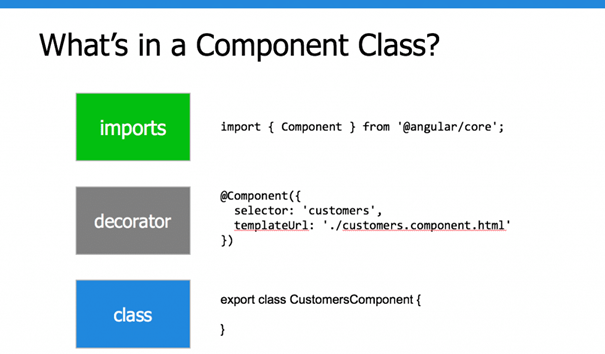
\includegraphics[width=0.8\textwidth]{pics/Komponenten_Klasse.png}
  \caption{Aufbau einer Komponente}
  \cite{AufbauKomponenteBild}
\end{figure}

Der Aufbau eines Bausteins ist immer gleich, ganz gleich welche Komponente geschrieben wird. Natürlich können einige Aspekte hinzugefügt werden, doch die Gesamtstruktur sieht immer gleich aus. Das sorgt für Konsistenz von Anfang an.

Services sind ein weiterer großer Bereich der Konsistenz in Angular. Diese sind ebenfalls wieder aufgebaut wie Bausteine. In den Konstruktor einer Service Klasse können alle Abhängigkeiten, die vom Service erfordert werden, eingefügt werden.

\begin{figure}[H]
  \centering
  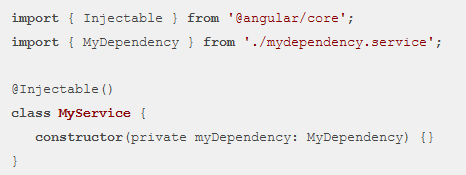
\includegraphics[width=0.8\textwidth]{pics/Code_Service.png}
  \caption{Beispielcode einer Service-Klasse}
\end{figure}

\subsubsection{Produktivität}
Die Produktivität rückt durch die Konsistenz in den Vordergrund. Denn der Entwickler muss sich keine Gedanken darüber machen, ob er die Dinge auf die „richtige Weise“ macht. Komponenten und Services sehen gleich aus, wiederverwendbarer Anwendungscode wird in Serviceklassen abgelegt und ES-Module organisieren zugehörige Funktionen und ermöglichen, dass der Code self-contained und self-responsible ist. Daten werden mithilfe von Eingabeeigenschaften an Komponenten übergeben und lassen sich durch Ausgabeeigenschaften weitergeben.

\subsubsection{Wartbarkeit}
Angular hat den Vorteil, dass es von einer großen Community, mit Hilfe von Open-Source-Beiträgen regelmäßig erweitert. Den größten Teil der Erweiterungen trägt allerdings Google bei. Es ist nie sicher, wie lange ein bestehendes System genutzt werden kann. Angular hat den Vorteil, dass sich Google über die Auswirkungen von etwaigen Änderungen bewusst ist und da Google Angular selbst in Projekten verwendet, gibt es die Sicherheit, dass sich nichts schlagartig verändert oder die Wartung eingestellt wird. Neben der Unterstützung durch das Angular Team, ist auch die beschriebene Konsistenz ein Vorteil für die einfache Wartbarkeit.

\subsubsection{Modularität}
Angular organisiert den Code in sogenannten „Buckets“. Komponenten, Services, Pipes oder Anweisungen müssen in einem oder mehreren Buckets organisieren. Die „Buckets“ werden in Angular als Module bezeichnet. Sie bieten die Möglichkeit, die Anwendungsfunktionalität zu organisieren und in Funktionen oder wiederverwendbare Abschnitte zu unterteilen. Module bieten außerdem noch viele andere Vorteile. 

\subsubsection{Frühzeitige Fehlererkennung}
TypeScript ist die Sprache zur Erstellung von Angular, dass bringt einige Vorteile mit sich:

\begin{itemize}
  \item TypeScript ist keine eigenständige Sprache und somit eine Obermenge von JavaScript. Es kann vorhandener ES JavaScript Code verwendet werden und der Code funktioniert einwandfrei.
  \item Außerdem unterstützt TypeScript die wichtigsten ES-Funktionen.
  \item Typen werden von TypeScript unterstützt, und sind für eine Frühzeitige Fehlererkennung enorm wichtig. Dadurch wird leichter erkannt ob etwas falsch übergeben oder verwendet wird.
  \item TypeScript Code kann direkt über den Browser debuggt werden.
  \item Bei TypeScript können ebenso Klassen und/oder funktionale Programmiertechniken verwendet werden.
\end{itemize}

Angular wurde ebenso mit dem hinter Gedanken an Testbarkeit entwickelt. Die Angular-CLI macht den Prozess des Komponententests und des End-to-End Tests sehr einfach. Standardmäßig wird Karma und Jasmine dafür verwendet. Zudem kann mit dem Befehl „ng test“ alle im Projekt vorhandenen Tests ausgeführt werden.

\cite{VorteileAngular}

\subsubsection{Nachteile von Angular}
\begin{itemize}
  \item Es gibt viele Wege in Angular das gleiche Ziel zu erreichen, deshalb ist es für den Programmierer oft schwer sich für den richtigen und effizientesten Weg zu entscheiden.
  \item Zudem sind die Lebenszyklusmethoden komplex, was sie nur schwer zu verstehen lässt.
  \item Das Nutzen von Direktiven ist für die Manipulation des DOM sehr hilfreich, jedoch ist die Erstellung nicht gerade einfach.
  \item Das Erlernen von Angular ist aufgrund von nicht vollständig ausreichender Dokumentation etwas schwieriger.
\end{itemize}
\cite{NachteileAngular}

\subsection{Angular Materials}
Um das Design der Anwendung zu vereinfachen, wurde Angular Materials verwendet. Angular Materials sind moderne, schlichte Designkomponenten, mit denen unter relativ geringem Aufwand optisch ansprechende Anwendungen gestaltet werden können, welche sich auch auf allen Anzeigegeräten mit geringem Zusatzaufwand umsetzen lassen. \cite{AngularMaterials}

Objekte sollen in einem drei-dimensionale Raum simuliert und eine natürliche, intuitive Darstellung und Interaktion ermöglicht werden. Bei der Entwicklung müssen dafür verschieden Prinzipien beachtet werden. 

\begin{itemize}
  \item Materialien besitzen eine einheitliche Höhe von 1dp, können aber in x- und y-Dimension verschieden sein.
  \item Der geworfene Schatten von Materialen ist je nach Höhe unterschiedlich.
  \item Materialien sind für die Darstellung von Inhalten, welche dynamisch veränderbar sind, zuständig. Es kann nur ein Teil von Materialien damit ausgefüllt werden, der Platz ist durch dessen Dimensionen beschränkt.
  \item Materialien sind Festkörper und können nur an freien Positionen eingesetzt werden. Ihre Transformationen sind, auf freien Platz im Raum, beschränkt.
  \item Sie dürfen ihre Form und Größe jederzeit ändern, wobei die zuvor genannten Einschränkungen zu beachten sind. Die Materialien sind trotzdem als fest anzusehen und dürfen nicht gefalten oder verbogen werden.
  \item Materialien können sich verbinden oder trennen.
\end{itemize}

Es werden von Angular Material bereits viele Designideen vorumgesetzt angeboten. Diese müssen oftmals nur als css-Klasse oder Direktive angefügt werden.

\begin{itemize}
  \item Theming: Das Farbschemata kann mittels scss-Mixins einfach geändert werden. Um komplexere Änderungen vorzunehmen, können eigene Mixins erstellt werden.
  \item Elevation helpers: Die z-Positionen können durch css-Klassen oder Mixins einfach dargestellt werden. Es gibt auch ein Mixin für Animationen bei Höhenänderung.
  \item Typography: font-size, -height und -weight sind von css-Klassen vorgegeben, mithilfe von Mixins können auch diese verändert werden.
\end{itemize}

\begin{lstlisting}[caption=Hinzufügen von Angular Materials]
  npm install --save @angular/material @angular/cdk @angular/animations
\end{lstlisting}

Mit diesem Befehl wird Angular Material zum Projekt hinzugefügt.
Material: Dieses Standardpaket enthält die Materialkomponenten.
CDK (Component Dev Kit): Dieses Paket stellt dem Entwickler, komponentenunabhängige Werkzeuge zur Verfügung.
Animations: Für erweiterte Animation, wird diese Paket benötigt.

Theme
Das Design von Angular Materials muss durch ein Theme definiert werden. Es kann eines der vorgefertigen verwendet oder auch eine eigenes definiert werden. Zur Auswahl bei den vorgefertigten Themes stehen:

\begin{itemize}
  \item deeppurple-amber.css
  \item indigo-pink.css
  \item pink-bluegrey.css
  \item purple-green.css
\end{itemize}
\cite{AngularMaterials}


\subsection{React}

\section{Auswahl der Technologie - Datenbank[SK]}
\setauthor{Simon Koll}
Die Datenbank spielt für das Projekt eine wichtige Rolle, daher wurden hier folgende Kriterien aufgestellt:

\begin{itemize}
  \item Das Projekt besteht aus Hard- und Software, die Daten sowohl abspeichern, als auch abfragen. Das kann je nach Anwendungsfall unterschiedlich sein.
  \item Vom Dashboard können beispielsweise Kennzeichen mit Gültigkeitsdauer, aber auch nur einfache NFC-Codes gesendet werden.
  \item In der Zukunft soll die Möglichkeit bestehen, weitere Zutrittsmöglichkeit hinzuzufügen. Daher muss sich die Datenbank der sich ändernden Datenstruktur anpassen können.
\end{itemize}

\subsection{Relationale Datenbanken}

Das Team befand sich vor der Entscheidung, ein relationales Datenbanksystem zu verwenden, oder ein nicht relationales Datenbanksystem.
Die größten Unterschiede hierbei sind, dass bei relationalen SQL-Datenbanken den gespeicherten Daten Tabellen vorgegeben sind, das sogenannte Schema. Das ist bei NoSQL-Datenbanken ebenfalls möglich, jedoch optional.
Relationale Datenbanken verfolgen das ACID-Prinzip. ACID steht für

\begin{itemize}
  \item \textit{Atomicity}
  \subitem Alle Änderungen der Datenbank werden als einzige Operation verarbeitet. Entweder werden alle Änderungen wie Inserts, Updates usw. durchgeführt, oder keine davon.
  \item \textit{Consistency}
  \subitem Zu Beginn und zum Ende jeder Transaktion sind die Daten konsistent.Beispielsweise bei einer Geldüberweisung, ist bei "Consistency" die Gesamtsumme der Geldmittel auf beiden Konten am Anfang und am Ende jeder Transaktion gleich.
  \item \textit{Isolation}
  \subitem Andere Transaktionen haben keine Einsicht in die Transaktion. Isolation bedeutet also, dass parallel laufende Transaktionen sich wie serialisierte verhalten.
  \item \textit{Durability}
  \subitem Die Daten bleiben nach Ende der Transaktion bestehen und werden auch bei einem kompletten Systemausfall nicht revidiert.
\end{itemize}
\cite{ACID}

\subsection{MongoDB}
Das Team entschied sich für eine der bekanntesten NoSQL-Datenbanken, \textbf{MongoDB}. Diese bietet einige Vorteile gegenüber den relationalen SQL-Datenbanken:

\begin{itemize}
  \item \textit{Skalierbarkeit: } MongoDB Datenbanken zeichnen sich durch ihre ausgezeichnete horizontale Skalierbarkeit aus. Horizontale Skalierbarkeit bedeutet, dass die Datenbank sich problemlos über mehrere Server verteilen kann, ohne die Funktionsfähigkeiten zu beeinträchtigen.
  \item \textit{Verfügbarkeit: } Die Datenbank muss immer zur Verfügung stehen, da  Abfrage ausgeführt wird.
  \item \textit{Flexibilität: } Da das Projekt weiterentwickelt werden kann, muss die Datenbank sich anpassen können.
\end{itemize}
\cite{VorteileMongoDB}
\section{Auswahl der Technologie - Kennzeichenerkennung[SK]}
\setauthor{Simon Koll}
Das Herz von APERTA ist die Kennzeichenerkennung. Dieses Alleinstellungsmerkmal separiert das Projekt von möglicher Konkurrenz. Dabei spielen Faktoren wie der Aufnahmewinkel der Kamera, die Distanz zum Kennzeichen, sowie die Lichtsituation eine entscheidende Rolle. Weiters muss aus den Einzelbildern der Kamera das Kennzeichen erkannt werden und danach die Buchstaben aus dem Bild extrahiert werden. Um dies zu vollbringen, werden 2 Libraries verwendet.
\subsection{OpenCV: } OpenCV steht für Open Source Computer Vision und ist eine frei Zugängliche Library, welche meist in Bereichen wie Machine Learning oder Machine Vision ihren Einsatz findet. Unternehmen können kostenlos auf die Bibliothek zugreifen, sie verändern und weiterentwickeln. Die Basis bilden die mehr als 2500 klassischen und neuen Algorithmen für das maschinelle Sehen. Diese haben unterschiedliche Spezialisierungen, wie unter anderem die Erkennung von Gesichtern, Objekten und Kamerabewegungen, die Generierung von 3D-Modellen, Ähnlichkeiten in Bildern zu finden, sowie Markierungen in Augmented Reality anzuzeigen. Zu den mehr als 18 Millionen Downloads und mehr als 47.000 Benutzern oder Benutzerinnen zählen meist Unternehmen, Forschungsgruppen oder Regierungsstellen. Bekannte Namen hier sind Google, Microsoft, Intel oder Sony.\cite{AboutOpenCV}
OpenCV hat eine modulare Struktur, was bedeutet, dass das Paket mehrere gemeinsam genutzte oder statische Bibliotheken enthält. Die folgenden Module sind verfügbar:
\begin{itemize}
    \item Kernfunktionalität (core) - ein kompaktes Modul, das grundlegende Datenstrukturen definiert, darunter das dichte mehrdimensionale Array Mat und grundlegende Funktionen, die von allen anderen Modulen verwendet werden.
    \item Bildverarbeitung (imgproc) - ein Bildverarbeitungsmodul, das lineare und nichtlineare Bildfilterung, geometrische Bildtransformationen (Größenänderung, affines und perspektivisches Warping, generisches tabellenbasiertes Remapping), Farbraumkonvertierung, Histogramme usw. umfasst.
    \item Videoanalyse (Video) - ein Videoanalysemodul, das Algorithmen zur Bewegungsschätzung, Hintergrundsubtraktion und Objektverfolgung umfasst.
    \item Kamerakalibrierung und 3D-Rekonstruktion (calib3d) - grundlegende Geometriealgorithmen für mehrere Ansichten, Einzel- und Stereokamerakalibrierung, Objektposenschätzung, Stereokorrespondenzalgorithmen und Elemente der 3D-Rekonstruktion.
    \item 2D Features Framework (features2d) - Erkennung auffälliger Merkmale, Deskriptoren und Deskriptor-Matcher.
    \item Objekterkennung (objdetect) - Erkennung von Objekten und Instanzen der vordefinierten Klassen (z. B. Gesichter, Augen, Tassen, Menschen, Autos usw.).
    \item High-Level-GUI (highgui) - eine leicht zu bedienende Schnittstelle zu einfachen UI-Funktionen.
    \item Video I/O (videoio) - eine einfach zu bedienende Schnittstelle für Videoaufnahmen und Videocodecs.
    \item Einige andere Hilfsmodule, wie z.B. FLANN- und Google-Test-Wrapper, Python-Bindings, und andere.
\end{itemize}
 \subsection{Tesseract: } Tesseract ist eine Texterkennungs-Engine welche von Google entwickelt wird. 

 Optische Zeichenerkennung oder Optical Character Reading (OCR) ist die elektronische oder mechanische Umwandlung von Bildern mit getipptem, handgeschriebenem oder gedrucktem Text in maschinell kodierten Text, sei es aus einem gescannten Dokument, einem Foto eines Dokuments, einem Szenenfoto (z. B. der Text auf Schildern und Werbetafeln in einem Landschaftsfoto) oder aus einem Untertiteltext, der einem Bild überlagert ist (z. B. aus einer Fernsehsendung).
 \cite{ocrWiki}

Um besser zu verstehen, wie OCR funktioniert, hilft dieses Prozessdiagramm in der folgenden Abbildung. Aus Sicht von Endbenutzern oder Endbenutzerinnen ist der OCR-Prozess einfach: Er verarbeitet das Bild und erhält den bearbeitbaren Text.
\begin{figure}[H]
  \centering
  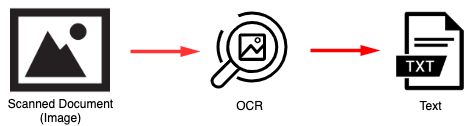
\includegraphics[width=10cm]{pics/OCR-Prozessdiagramm.png}
  \caption{Prozessdiagramm der Optische Zeichenerkennung}
  \cite{introToTesseract}
\end{figure}
 Tesseract bietet die Möglichkeit, Text aus Bildern zu extrahieren. Dies kann in vielen verschiedenen Programmiersprachen erfolgen, oder über eine graphische Nutzeroberfläche eines Drittanbieters.\cite{AboutTesseract} Unterstützt wird Tesseract durch einen Python-Wrapper mit dem Namen \textbf{pytesseract}, welcher Bilder wie .jpeg, .png, .gif und viele mehr laden kann, sowie den gelesenen Text ausgeben kann, anstatt ihn in einer Datei abspeichern zu müssen.\cite{AboutPyTesseract}
 
\section{Auswahl der Technologie - Backend[SK]}
\setauthor{Simon Koll}
\subsection{Anforderungen an das Backend}
Für das Backend kamen mehrere Technologien in Frage, wie unter anderem Java, JavaScript, Python, PHP, C$\sharp$, und viele mehr.
Um das Backend zu realisieren, muss die Technologie einige bestimmte Eigenschaften besitzen.\cite{CompareBackendLanguage}
\begin{itemize}
    \item \textit{Java:}
    \subitem Die Vorteile von Java liegen in der Fehlerbehandlung, sowie in Bereichen wie Multithreading und Performanz. Die strikte Fehlerbehandlung führt dabei aber zum Verlust von Flexibilität und Kompaktheit des Codes.
    \item \textit{JavaScript:}
    \subitem Die Syntax von JavaScript ähnelt der von Java. Entwickelt als Scripting-Sprache für HTML, ist JavaScript einfach zu lernen und zu benutzen. Bei der Entwicklung von Websites kann JavaScript direkt in den Quellcode der HTML-Seite eingearbeitet werden. Aber auch im Backend-Bereich kann mit NodeJS in JavaScript entwickelt werden.
    \item \textit{Python:}
    \subitem Python ist eine der mit Abstand am leichtesten zu lesenden Programmiersprachen. Die flache Hierarchie ermöglicht ein einfaches Verständnis von Programmen und Codestücken. Weiters macht Python Entwickler oder Entwicklerinnen auf Fehler aufmerksam, wenn dieser nicht ausdrücklich ignoriert werden soll.
    Jedoch ist Python manchmal langsamer in der Ausführung, als die konkurrierenden Sprachen. Zusätzlich ist durch die Verwendung von Leerzeichen zur Einrückung ein häufiger Fehlergrund hinzugekommen.
    \item \textit{PHP:}
    \subitem Die PHP Syntax erinnert an eine Mischung aus C, Java und Perl. Das Ziel von PHP ist es, Entwickler oder Entwicklerinnen schnell und einfach dynamisch generierte Webpages bauen zu lassen. Die vermischte Syntax ist jedoch etwas chaotisch, darum ist es leicht, sich in falschen Angewohnheiten zu verirren und Sicherheitslücken offen zu lassen.
  \end{itemize}
  Aufgrund vorhandener Vorkenntnisse standen für das Team 3 der oben genannten Technologien zur Auswahl:

  \begin{itemize}
    \item Java,
    \item JavaScript und
    \item Python
  \end{itemize}

  \subsection{Verwendung von NodeJS}
  Von diesen konnte sich JavaScript durchsetzen. Die Gründe dafür waren:\cite{WhyNodeJs}
  \begin{itemize}
    \item NPM:
    Der NPM oder \textit{Node Package Manager}, ist ein Paketmanager für JavaScript, welcher bei NodeJS standardmäßig mitgeliefert wird. Bei NPM werden wiederverwendbare Programmteile veröffentlicht. Diese können mittels des NPM eingenen Command Line Interfaces installiert werden. Weiters bietet der NPM eine integrierte Versionsverwaltung der Pakete, sowie eine Verwaltung der Abhängigkeiten.
    In diesem Projekt wurden beispielsweise die Module \textit{express} und \textit{mongodb} verwendet. \\
    \textit{express} ist ein Framework, welches vor allem in NodeJS Projekten verwendet wird. Die Vorteile von Express sind unter anderem die dem Team bereits bekannte Programmiersprache JavaScript, die Unterstützung der Google V8 engine für bessere Performance, die Robustheit bei einer Vielzahl an HTTP-Anfragen, sowie die einfache Einbindung weiterer Module und Drittanbieterapplikationen. \cite{WhyExpress}\\
    \textit{mongodb} stellt Entwicklern pder Entwicklerinnen eine API zur Verfügung, welche die Nutzung einer MongoDB-Datenbank stark vereinfacht.
    \item Verwendung einer NoSQL Datenbank:
    Aufgrund des Formates, mit dem die Daten aus dem Frontend kommen, bat sich eine nicht relationale Datenbank für das Team an. Die dokumentenorientierte Datenbank MongoDB ist bekannt für ihre hohe Verfügbarkeit, sowie für die gute Skalierbarkeit.
    \cite{WhyMongoDB}
    \item Behandlung von JSON:
    NodeJS zeichnet sich durch seine einfache Verwendung von JSON-Daten aus. Diese können ohne Parsing oder andere Konvertierungen verarbeitet und darauf zugegriffen werden. Dank NodeJS können JSON Objekte mittels REST-API Anfragen direkt für den Client bereitgestellt werden.
    Dank NodeJS kann eine einfache Verbindung zwischen Frontend-Clients und dem Backend-Server geschaffen werden.
  \end{itemize}

\section{Auswahl der Technologie - Hardware[SK]}
\setauthor{Simon Koll}
\subsection{Anforderungen an die Hardware}
Das Projekt sollte so vielseitig wie möglich, jedoch auch so kompakt wie möglich sein. Dazu musste auf kleine Komponenten gesetzt werden. Diese sollen dennoch leistungsfähig genug sein, um jede der drei Zugangsmöglichkeiten parallel zu verwalten.
\subsubsection{Raspberry Pi}
Die Wahl des Herzstückes fiel auf einen Raspberry Pi.
Der Raspberry Pi ist ein vollwertiger Computer, welcher etwas größer als eine Kreditkarte ist. Er besitzt alle bekannten Anschlüsse eines normalgroßen PCs, wie HDMI-Ausgänge für Monitore, USB-Ports für Peripherie wie Maus, Tastatur oder Webcams, sowie einen LAN-Port für eine kabelgebundene Netzwerkverbindung.
Als Betriebssystem des Raspberry Pi wurde das vom Hersteller empfohlene Raspbian OS verwendet. Dieses bietet eine grafische Benutzeroberfläche, sowie die Möglichkeit den Raspberry auch ohne angeschlossenen Monitor betreiben zu können. \cite{WhatIsRaspberryPi}
\begin{figure}[H]
  \centering
  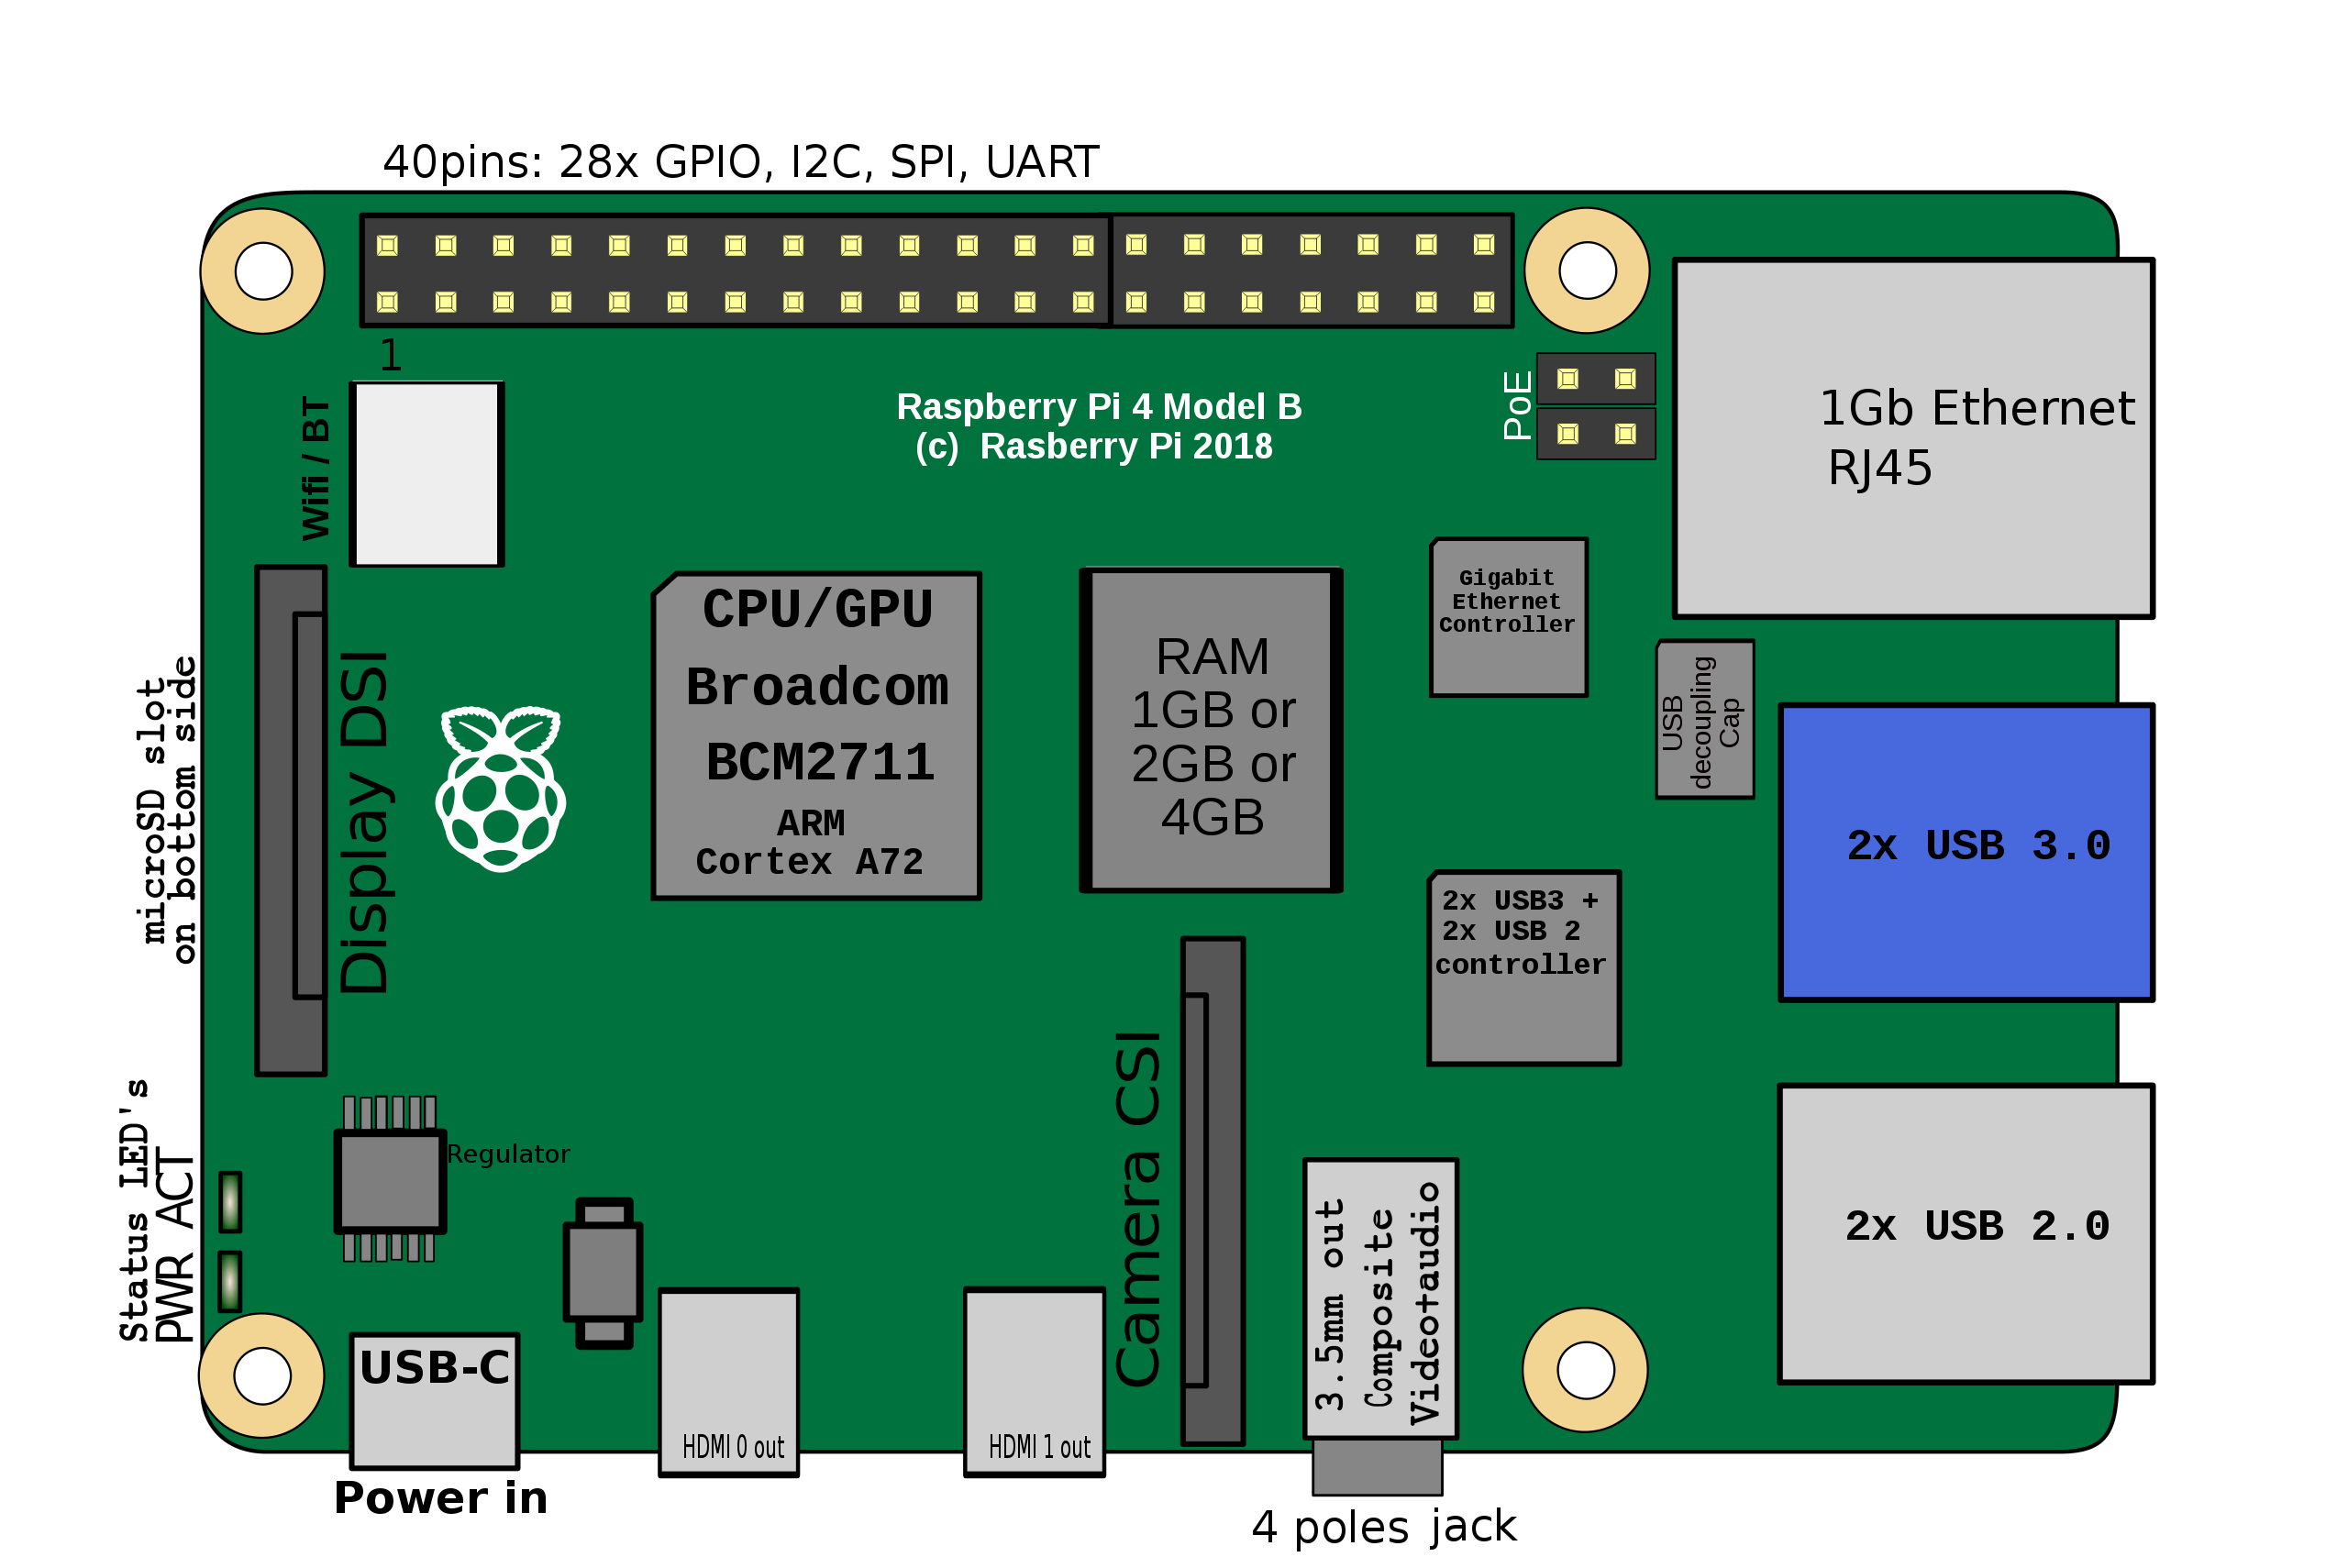
\includegraphics[width=10cm]{pics/2560px-RaspberryPi_4_Model_B.svg.png}
  \caption{Komponenten eines Raspberry Pi}
  \cite{RaspberryImage}
  \end{figure}


Auszeichnungsmerkmale des Raspberry Pi sind unter anderem die geringen Anschaffungskosten von ab EUR 35,00, sowie seine leistungsstarken Komponenten.\\
%\textbf{Bestandteile des Raspberry Pi} 
\begin{table}[H]
  \centering
  \caption{Übersicht der Komponenten des Raspberry Pi \cite{RaspySpecs}}
  \label{Komponenten des Raspberry Pi}
    \begin{adjustbox}{width=\textwidth}
      \begin{tabular}{lll}
      \hline
      \textbf{Komponente}                    & \textbf{Spezifikation}                                                    & \textbf{Besonderheiten}                    \\ \hline
      \multicolumn{1}{l|}{\textbf{Prozessor}} &
        \begin{tabular}[c]{@{}l@{}}Broadcom BCM2711\\ - Quad Core Prozessor @ 1.5GHz\end{tabular} &
        \begin{tabular}[c]{@{}l@{}}ARM Architektur\\ 64-Bit SoC\end{tabular} \\ \hline
      \multicolumn{1}{l|}{\textbf{RAM}}      & 1GB, 2GB, 4GB oder 8GB LPDDR4 SDRAM                                                          & Tatktung von 3200MHz                       \\ \hline
      \multicolumn{1}{l|}{\textbf{USB}}      & \begin{tabular}[c]{@{}l@{}}2 USB 3.0 Ports\\ 2 USB 2.0 Ports\end{tabular} &                                            \\ \hline
      \multicolumn{1}{l|}{\textbf{GPIO}}     & 40 Pin Header                                                             & Abwärtskompatibel mit Vorgängermodellen    \\ \hline
      \multicolumn{1}{l|}{\textbf{Display}}  & 2 micro-HDMI Ports                                                        & jeweils bis zu 4k60 möglich                \\ \hline
      \multicolumn{1}{l|}{\textbf{Speicher}} & Micro-SD Kartenslot                                                       & Speicherplatz für Betriebssystem und Daten \\ \hline
      \multicolumn{1}{l|}{\textbf{Strom}} &
        \begin{tabular}[c]{@{}l@{}}5V Eingang über USB-C Port\\ 5V Ausgang über GPIO-Header\end{tabular} &
        Anforderung an Stromquelle: mindestens 3A \\ \hline
      \end{tabular}
    \end{adjustbox}
  \end{table}
Der Raspberry Pi ist einer der am weitest verbreiteten Ein-Platinen-Computer der Welt. Trotz der im Verhältnis zu größeren Systemen schwachen Leistung wurde er im Jahr 2020 mehr als 7 Millionen mal verkauft worden. Daraus ergibt sich ein Marktanteil von allen PCs von 2.69\%.
Für ein ausgewogenes Verhältnis zwischen Kompaktheit und Leistung wurde auf einen Raspberry Pi 4 Model B in der Ausführung mit 4GB Arbeitsspeicher zurückgegriffen. Weiters waren die Anschaffungskosten von etwa 100\$ ein Grund für die Auswahl. \cite{RaspyMarketShare}

\textbf{Kernkomponenten des Raspberry Pi}\\
\textit{GPIO-Header}\\
Eine der Kernkomponenten, die den Raspberry Pi von anderen PC-Systemen unterscheidet, ist der "GPIO-Header". GPIO steht für General Purpose Input / Output, und kann wörtlich zu "Allzweckeingabe bzw. -ausgabe" übersetzt werden. Sie bezeichnen selbst programmierbare Ein- und Ausgänge, die auf dem Raspberry Pi als angelötete Pins zur Verfügung stehen.
Der Raspberry kann über diese Schnittstellen digitale Signale von außen annehmen, sowie auch Signale abgeben.
Der Raspberry Pi in der Ausführung Model 4 B hat einen 40-köpfigen GPIO-Header in Form einer Stiftleiste mit zwei Reihen. Davon gibt es einige GPIOs mit bestimmten Zusatzfunktionen, wie I2C, SPI oder einer seriellen Schnittstellen. Weiters gibt es Pins, welche vom Raspberry eine +5V-Spannung, eine +3.3V Spannung, oder die Möglichkeit der Erdung liefern.\\ \\
\textit{GPIO-Belegung und elektrische Eigenschaften}\\
Grundsätzlich kann in elektronischen Systemen auf elektrische Eigenschaften zurückgegriffen werden, die beobachtet werden müssen. Oft sind diese Eigenschaften Grenzwerte des Systems, welche nicht überschritten werden dürfen. Wird dies ignoriert, kann das System nach Start beschädigt werden und im weiteren Verlauf Defekte aufweisen.
Die Eingangsspannung des Raspberry Pi beträgt zwar 5V, jedoch arbeitet der Prozessor selbst nur mit 3.3V. Daher haben auch die GPIOs nur 3.3V zur Verfügung. Dies gilt für die Ausgangsspannung, jedoch auch für die Eingangsspannung, da sonst der Chip des Raspberry Pi beschädigt werden kann. 
\begin{figure}
  \centering
  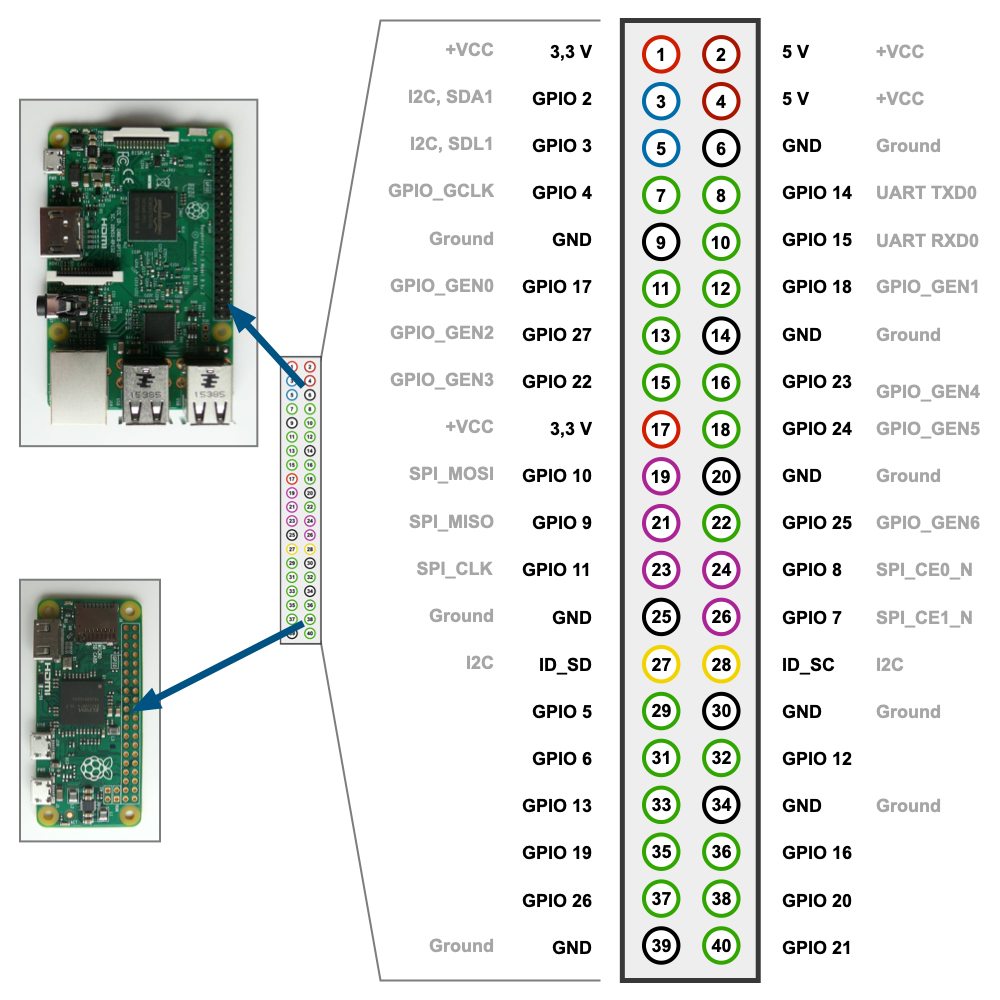
\includegraphics[width=10cm]{pics/GPIO.png}
  \caption{Belegung der GPIOs eines Raspberry Pi Model 4B / Raspberry Pi Zero}
  \cite{GPIOLayout}
\end{figure}
GPIOs sind empfindliche Schnittstellen, denn sie können schon bei geringen Stromstärken Schaden nehmen. Theoretisch ist eine Stromstärke von 16mA (Milliampere) möglich, wobei diese nie benötigt wird, da die GPIOs schon mit einer Stromstärke von 0.5mA geschalten werden können. Um die Langlebigkeit des Raspberry Pi zu gewährleisten, sollten nie mehr als 8mA von einem GPIO abgegeben werden. 
Es gibt jedoch Ausnahmen, wie die +5V-Pins. Diese bieten für externe Schaltungen eine Spannung bis zu 5V an, sind jedoch ebenfalls bei der Stromentnahme begrenzt. Hier wird mit etwa 25mA pro 5V-Pin gerechnet. Sollte dies für eine Schaltung nicht ausreichen, kann auf externe Stromquellen zurückgegriffen werden, wie eine Stromversorgung über ein separates Netzteil mit USB-Anschluss, oder die Versorgung über einen der verfügbaren USB-Ports des Raspberry Pi selbst. 

\cite{GPIO}
\subsubsection{NFC-Leser}
\subsubsection{Numpad [DH]}
Das Numpad ermöglich dem Benutzer die Eingabe eines 6-stelligen Zahlencodes. Dazu wird bei APERTA ein übliches Nummernfeld angeschlossen, der eingegeben Code wird dann mit den vorhandenen Codes in der Datenbank geprüft und abgeglichen. Stimmen die Zahlenkombinationen überein so öffnet sich das Garagentor. Zur Überprüfung wird der eingegebene Code auf dem LCD angezeigt. So kann sich vergewissert werden, dass keine falschen Zahlen eingegeben werden. Sollte doch eine falsche Kombination eingegeben worden sein, wird auf dem Display eine Fehlermeldung ausgegeben.

\begin{figure}
  \centering
  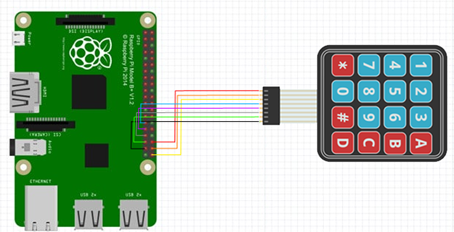
\includegraphics[width=0.8\textwidth]{pics/Nummerfeld.png}
  \caption{Abbildung eines Nummernfelds}
  \cite{Nummernfeld}
\end{figure}
\subsubsection{Kamera}
Die Kamera ermöglicht dem Raspberry Pi, die Kennzeichen zu sehen und darauf die Kennzeichen zu erkennen. Dazu wird bei APERTA eine handelsübliche Webcam verwendet, die über einen der beiden USB 3.0 Ports am Raspberry angeschlossen wird.
Um genug Auflösung für die Kennzeichenerkennung zu gewährleisten, wurde auf eine Webcam zurückgegriffen, welche mit bis zu 1920 Pixeln mal 1080 Pixeln aufnehmen kann.
Alternativ wäre auch eine Raspberry Pi Camera möglich gewesen, jedoch wurde die aufgrund ihres kurzen Flachbandkabels nicht verwendet, um die Kamera auch in größere Entfernung vom Raspberry Pi nutzen zu können.
\begin{figure}[H]
  \centering
  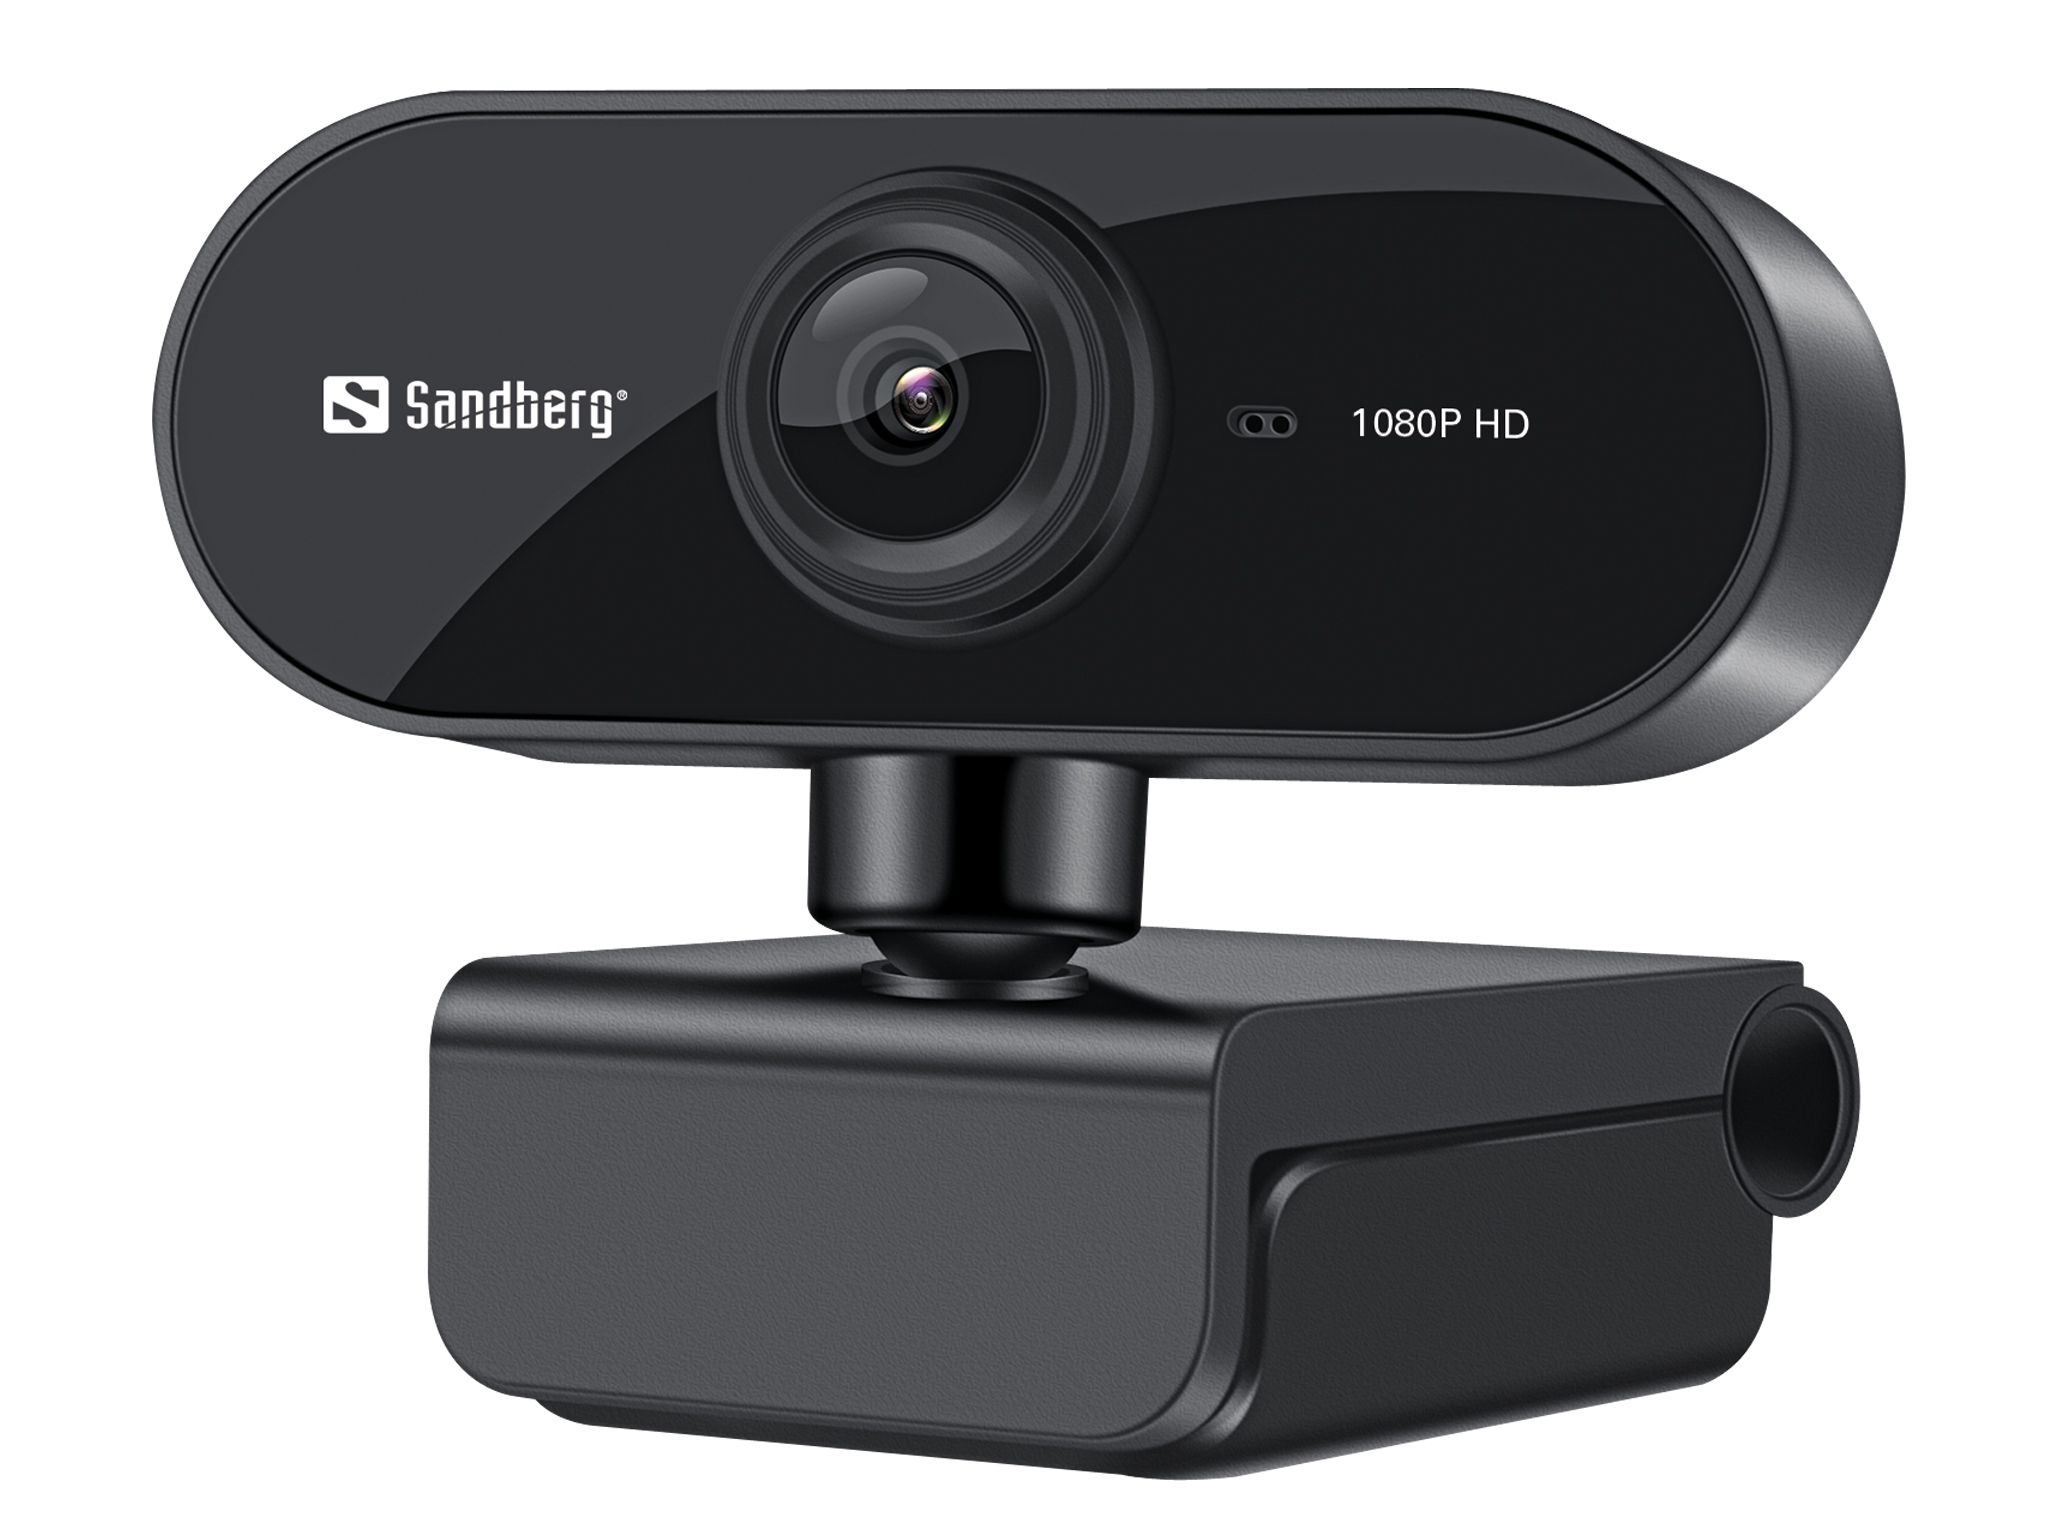
\includegraphics[width=8cm]{pics/Webcam.jpg}
  \caption{Webcam mit gleichen Spezifikationen}
  \cite{Webcam}
\end{figure}

\begin{figure}[H]
  \centering
  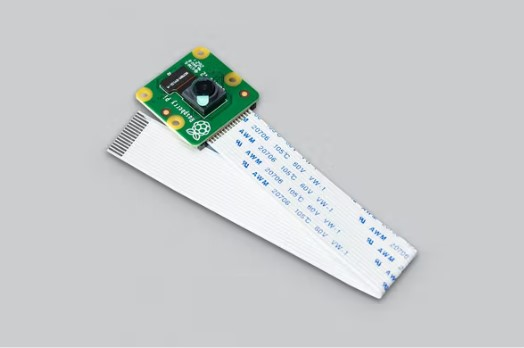
\includegraphics[width=8cm]{pics/RaspberryPiCameraModule2.jpg}
  \caption{Raspberry Pi Camera Module 2}
  \cite{PiCamera}
\end{figure}

\subsubsection{Display}
Um dem Nutzer oder der Nutzerin vor der Garage mitzuteilen, was gerade geschieht, wird ein Display verwendet, auf dem mitgeteilt wird, ob die Kombination, welche auf dem Nummernfeld eingegeben wurde korrekt ist, oder ob die NFC-Karte autorisiert ist.
Da auf diesem Display nur kurze Textausgaben angezeigt werden, fiel die Entscheidung auf ein LCD-Display, welches in zwei Zeilen beschrieben werden kann. Dieses bat zudem weitere Vorteile, wie die geringen Kosten von EUR 9,00 pro Stück, die Spannungsversorgung durch den Raspberry Pi selbst, sowie die einfache Möglichkeit, Text darauf auszugeben.
Im Lieferumfang des Displays war zudem ein I2C Serial Adapter, welcher durch seine 4 benötigten Ports um 8 Pins auf dem Raspberry Pi weniger braucht, als das direkt angeschlossene Display.
\cite{DifferentConnectionTypesDisplay}
\begin{figure}[H]
  \centering
  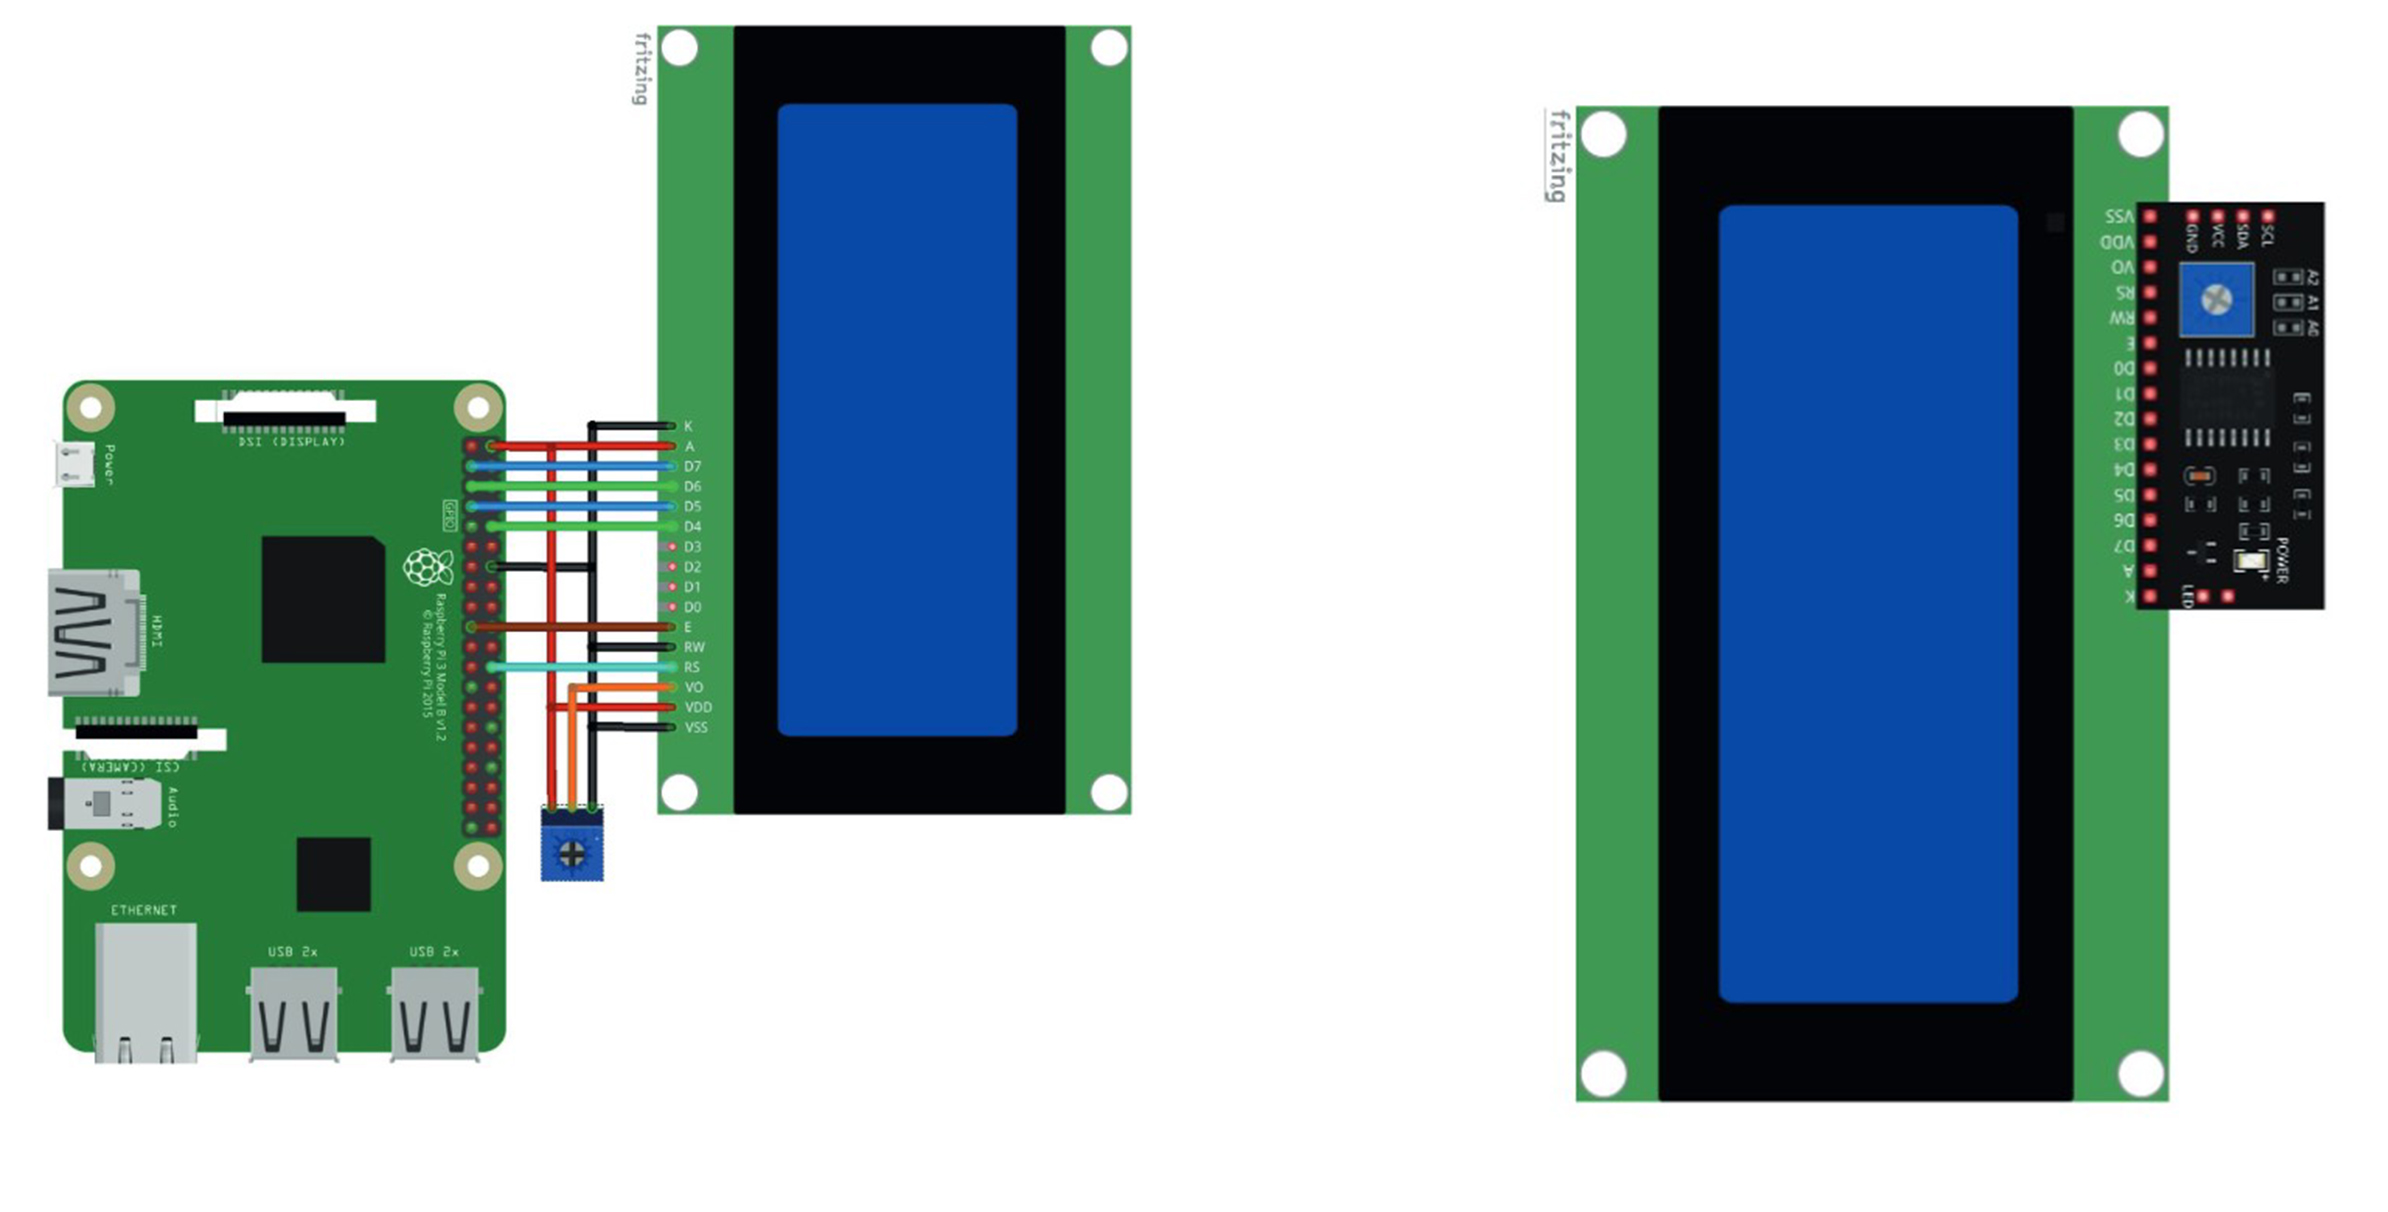
\includegraphics[width=15cm]{pics/DisplayComparison.jpg}
  \caption{Display direkt angeschlossen / Display über I2C Adapter angeschlossen}
\end{figure}
Die technischen Daten des Displays lauten:
\begin{itemize}
  \item 4 Zeilen zu je 20 Zeichen beschreibbar
  \item Blaue Hintergrundbeleuchtung
  \item 5V Versorgungsspannung
\end{itemize}
\cite{RaspberryDisplay}

 \subsubsection{Relais}
Handelsübliche Garagentore werden mit einer Spannung von 230 Volt betrieben. Der Raspberry Pi kann diese nicht direkt ansteuern, da die Spannung die interne Elektronik des Pi zerstören würde. Dennoch ist es nötig, wie bei einem Schalter den Steuerstromkreis des Garagentores zu schließen, um den Öffnungsmechanismus zu aktivieren. Um dies zu erreichen, wird ein Relais verwendet, welches in den externen Stromkreis geschalten wird und wie eine Brücke den Stromkreis schließen kann. Ein Relais besteht aus einer Spule aus Draht und einem Metallkern. Wird Strom durch den Draht geschickt, wird der Kern magnetisiert. Ohne Strom verschwindet das Magnetfeld des Kerns wieder.

Das Relais ist ein Elektromagnet, welcher durch den Steuerkreis einen Eisenanker zu sich zieht und somit den Arbeitsstromkreis schließt. Der Arbeitsstromkreis kann unabhängig vom Steuerkreis aufgebaut sein und auch unterschiedliche Spannungen und Stromstärken besitzen. Wichtig ist nur, dass das richtige Relais für den Arbeitskreis verwendet wird. Im Fall diese Projektes wird ein Relais verwendet, welches für bis zu 250 Volt Gleichstrom des Arbeitskreises verwendet werden kann.
\cite{Relais}
\begin{figure}[H]
  \centering
  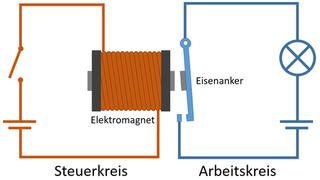
\includegraphics[width=8cm]{pics/Relais.png}
  \caption{Funktionsweise eines Relais als Schema}
  \cite{RelaisBild}
\end{figure}


\subsubsection{Steuerung der Hardware}
Um die Komponenten miteinander zu verbinden, war eine Programmiersprache notwendig, die mit den über GPIOs angeschlossenen Bauteilen kommunizieren kann. Dazu gab es eine Handvoll von Programmiersprachen, welche für die Entwicklung von Projekten mit dem Raspberry Pi in Frage kamen.

\begin{itemize}
  \item \textit{Scratch: }Scratch ist eine baukastenartige Programmiersprache, bei der Befehlsblöcke mithilfe der Maus aneinander angereiht werden. Entwickelt vom MIT Media Lab, richtet sich Scratch an Programmierneulinge und Kinder, welche es unterstützen soll, programmieren zu lernen, Code lesen und verstehen.
  \item \textit{Python: }Python zählt zu den meistverwendeten Programmiersprachen in Verbindung mit dem Raspberry Pi. Es zeichnet sich durch seine einsteigerfreundliche Syntax und die riesige Community aus, welche es ermöglicht, auf eine Vielzahl an Frameworks und Libraries zurückzugreifen. Python beschränkt sich dabei nicht auf einen bestimmten Einsatzbereich, sondern kann für die Entwicklung von graphischen Nutzeroberflächen, im Webdevelopment, zum Trainieren von Künstlichen Intelligenzen sowie für Automatisierung verwendet werden.
  \item \textit{JavaScript: } JavaScript ist nicht nur eine Erweiterung von HTML als Scripting Sprache, sondern viel mehr eine eigenständige, umfangreiche Programmiersprache. Sie wird meistens mit Webentwicklung in Verbindung gebracht, ist jedoch auch fähig, bereits bestehende Applikationen zu erweitern.
  \item \textit{Java: } Java ist eine der vielseitigsten Programmiersprachen, da sie erlaubt, unabhängig von Betriebssystem zu entwickeln, ohne den Code für jede Plattform verändern zu müssen. Mit mehr als 3 Milliarden Geräten, auf denen Java läuft, ist sie eine der meist verbreiteten Programmiersprachen.
  \item \textit{C: } C ist einer der stärksten Konkurrenten von Java. Raspbian OS, das Betriebssystem des Raspberry Pi, wurde beispielsweise in C geschrieben. C zeichnet sich durch einen klar strukturierten Programmierstil und die Möglichkeit, Arbeitsspeicher direkt anzusprechen, aus. Die Haupteinsatzgebiete von C sind die Entwicklung von Betriebssystemen und Compilern.
  \item \textit{C++: } Verglichen mit C, kann sich C++ mit objektorientierter Programmierung auszeichnen. Die Kombination aus prozeduraler und objektorientierterer Programmierung machen C++ zu einer Allzwecklösung, mit welcher von Betriebssystemen über Spiele bis hin zu Webbrowsern alles entwickelt werden kann.
  \item \textit{Perl: } Die Perl Org. hat mit Perl eine Sprache entwickelt, welche für fast jede Aufgabe, die mit C oder C++ Libraries zu tun hat, geeignet ist. Die große Auswahl an Libraries und Modulen sprechen trotz der geringen Bekanntheit für Perl, welche weiters für die Webentwicklung, Systemadministration, GUI-Entwicklung und vielem mehr verwendet werden kann.
  \item \textit{Erlang: } Erlang ist eine relativ unbekannte Sprache, da sie meist für Industrieapplikationen verwendet wird. Auszeichnungsmerkmale von Erlang sind beispielsweise die Fähigkeit, skalierbare Echtzeitsysteme zu entwickeln. Auch bei dezentralisierten Systemen ist Erlang eine gute Wahl, da das Programm bei Ausfall eines Rechners aus dem Cluster problemlos weiter arbeiten kann. Verwender sind unter anderem Banken und Telekommunikationsunternehmen.
\end{itemize}
\cite{RaspberryProgramming}\\
Durch die einfache Möglichkeit, mit den GPIOs zu arbeiten, sowie der einfach verständlichen Syntax, wurde Python verwendet. Das Team konnte somit zusätzlich auf bereits bestehende Kenntnisse aufbauen.

\begin{spacing}{1}
	\chapter{Lösungsansätze}\label{chapter:solution}
	\end{spacing}
	\section{Profil Management}
\setauthor{David Hauser}
\section{Webshop}
\setauthor{Benjamin Golic}
\section{Automatic Number Plate Recognition (ANPR)[SK]}
\setauthor{Simon Koll}
\label{lsg:def:anpr}
Die Kennzeichenerkennung stellt das Alleinstellungsmerkmal des Projektes dar. Der OpenCV-Python-Code für die Nummernschilderkennung umfasst drei Hauptschritte. Der erste Schritt ist die Erkennung von Nummernschildern. Die Konturfunktion wird verwendet, um die rechteckigen Objekte im Bild zu erkennen und das Nummernschild zu finden. Der zweite Schritt ist die Zeichensegmentierung. Sobald die Kontur das Nummernschild erkannt hat, müssen wir es ausschneiden und als neues Bild speichern. Und der letzte Schritt ist die Zeichenerkennung. Die optische Zeichenerkennung wird auf dem ausgeschnittenen Bild durchgeführt, um das Kennzeichen zu erkennen.

\subsection{Überprüfung der Kennzeichen}
Die erkannten Buchstaben werden genutzt, um eine Funktion aufzurufen, welche diese mit den zugelassenen Kennzeichen vergleicht. Dazu werden die zugelassenen Kennzeichen vom Server abgefragt, welcher diese aus der Datenbank lädt. Die Abfrage erfolgt über einen REST-Abfrage.
REST ist weder ein Protokoll, noch ein Standard. REST steht für REpresentational State Transfer, API für Application Programming Interface, welche gemeinsam eine Programmierschnittstelle bilden, mit der eine Anwendung mit einem Server kommunizieren kann. Dies wird meist mit dem HTTP-Protokoll genutzt, um Services über URLs zu erreichen. Dazu stehen die HTTP-Methoden GET, POST, PUT und DELETE zur Verfügung.
\begin{itemize}
    \item \textit{GET: } GET ist eine Methode, welche einen Inhalt eines Servers abruft.
    \item \textit{POST: } POST ist eine Methode, um vom Client Daten an den Server zu senden, welcher diese weiter verarbeiten und in die Datenbank speichern kann.
    \item \textit{PUT: } PUT bietet die Möglichkeit, bereits bestehende Daten zu ändern.
    \item \textit{DELETE: } DELETE bietet die Möglichkeit, bestehende Daten zu löschen.
\end{itemize}\cite{WhatIsREST}
Neben der Kennzeichenerkennung bietet das Projekt noch 2 weitere Zutrittsmöglichkeit, nämlich das Nummernfeld sowie die NFC-Funktionalität. Damit alle Zutrittsmöglichkeiten parallel funktionieren, wird mit der Bibliothek \textit{threading} parallel gearbeitet. Hiermit können mehrere Funktionen parallel gestartet werden. Dies kann beispielsweise wie folgt erfolgen: 
\begin{lstlisting}[language=Python, caption=Funktionsweise von Multiprocessing, label=lst:lsg:multiprocessing]
import time
from threading import Thread
    def funktion_1():
        while True:
            print("Funktion 1")
            time.sleep(1)
    
    
    def funktion_2():
        while True:
            print("Funktion 2")
            time.sleep(1)
    
    
    thread_1 = Thread(target=funktion_1)
    thread_2 = Thread(target=funktion_2)
    
    thread_1.start()
    thread_2.start()
\end{lstlisting}
\verb|thread_1| und \verb|thread_2| sind Threads, welche parallel ausgeführt werden. Sie bekommen als Parameter eine Funktion, welche ausgeführt werden soll, in diesem Fall \verb|funktion_1| und \verb|funktion_2|. Mit \verb|start()| werden die Threads gestartet.
    \cite{threading}
\section{Backend}
\setauthor{Simon Koll}
Der Server bildet das Rückgrat des Projektes. Hier werden die Daten aus der Datenbank abgefragt. Diese werden von einem Client über einen REST-Aufruf abgefragt. Der Server kann zudem die neu zugelassenen Kennzeichen in die Datenbank speichern.
\subsection{Oracle VM}
Der Server läuft auf einer Instanz einer Oracle Virtual Machine, ebenso die MongoDB-Datenbank. Die Oracle VM bietet die Möglichkeit, eine leistungsstarke Basis für den Server sowie die Datenbank bereitzustellen. Die technischen Daten der Instanz sind:
\begin{table}[ht]
    \caption{Technische Daten der Oracle VM Instanz}
    \label{tab:vm}
    \begin{tabular}{|l|llll}
    \cline{1-2}
    \textbf{Komponente} & \multicolumn{1}{l|}{\textbf{Wert}} &  &  &  \\ \cline{1-2}
    \textbf{CPU}        & 2 OCPU                             &  &  &  \\ \cline{1-1}
    \textbf{RAM}        & 16 GB                              &  &  &  \\ \cline{1-1}
    \textbf{Netzwerk}   & 1.4 GBit Bandbreite                &  &  &  \\ \cline{1-1}
    \end{tabular}
    \end{table}

    Im Vergleich zu anderen Cloudanbietern wie AWS, Microsoft oder Google, verwendet die Oracle Cloud Infrastructure, kurz OCI, anstelle von virtuellen CPUs sogenannte OCPUs. Jede vCPU ist als ein Hyperthread eines Intel Xeon-Kerns definiert. Ein Standard-Intel-Prozessorkern mit aktiviertem Hyperthreading hat 2 Threads.
\begin{figure}[H]
    \centering
    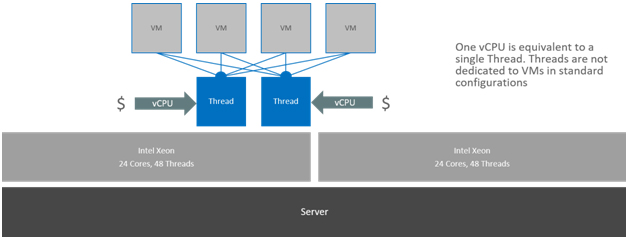
\includegraphics[width=0.8\textwidth]{pics/vCPU.jpg}
    \caption{Visualisierung von vCPUs}
    \cite{vcpuPic}
    \label{fig:vm:vCPU}
\end{figure}

    Eine OCPU ist definiert als die CPU-Kapazität, die einem physischen Kern eines Intel Xeon-Prozessors mit aktiviertem Hyperthreading oder einem physischen Kern eines Oracle SPARC-Prozessors entspricht.
    \begin{figure}[H]
        \centering
        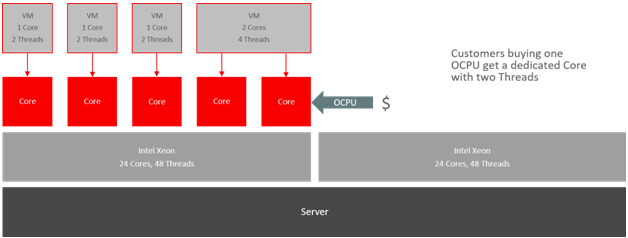
\includegraphics[width=0.8\textwidth]{pics/OCPU.jpg}
        \caption{Visualisierung von OCPUs}
        \cite{ocpuPic}
        \label{fig:vm:OCPU}
    \end{figure}
\cite{vcpuVsocpu}
\section{MongoDB}
Die Datenbank läuft auf der selben Oracle VM Instanz wie das Backend. Somit gibt es zwischen Server und Datenbank keine zusätzliche Latenz. Da MongoDB eine nicht relationale Datenbank ist, werden die Daten in sogenannten Collections anstelle von Tabellen abgespeichert. Je nach abzuspeichernder Zugangsmöglichkeit, verändert sich das Format der Daten.
Für ein Kennzeichen müssen die Daten wie folgt strukturiert sein:

\subsubsection{Kennzeichen}
\begin{lstlisting}[language=JSON, caption=Aufbau eines Kennzeichen in der Datenbank, label=lst:lsg:licenseplate]
    {
        "_id": "623f449cb8c1b2f4f64c4351",
        "licenseplate_id": 1,
        "licenseplate": "RO 108DV",
        "time_created": 1647252201,
        "active": true
    }
\end{lstlisting}
Das Attribut \verb|_id| wird automatisch generiert und ist ein eindeutiger Schlüssel, welcher die eindeutige Identifizierung eines Datensatzes darstellt. Mithilfe des \verb|licenseplate_id| wird eine eindeutige Kennzeichen Identifikationsnummer gespeichert. \verb|licenseplate| ist das Kennzeichen, welches vom Client übergeben wurde. \verb|time_created| ist die Zeit, zu der das Kennzeichen erstellt wurde. \verb|active| gibt an, ob das Kennzeichen der aktiv ist.

\subsubsection{Nummernfeld}
Bei einer Nummernfeld-Kombination sieht der Datensatz wie folgt aus:
\begin{lstlisting}[language=JSON, caption=Aufbau einer Nummernfeld-Kombination in der Datenbank, label=lst:lsg:numpad]
    {
        "_id": "622f181d35a3c2ce232acad9",
        "numpad_id": 1,
        "numpad_code": "123456",
        "time_created": 1647252201,
        "active": true
    }
\end{lstlisting}

\subsubsection{NFC}
Jede NFC-Karte hat eine eindeutige, 10-stellige Kartenidentifikationsnummer. Diese kann mittels eines RFID-Lesers ausgelesen werden. In der Datenbank werden die NFC-Informationen wie folgt gespeichert:
\begin{lstlisting}[language=JSON, caption=Aufbau einer NFC-Karte in der Datenbank, label=lst:lsg:nfc]
    {
        "_id": "622f781cfbd4e8de471a4035",
        "rfid_id": 3,
        "rfid_code": "01928384756",
        "time_created": "123456789",
        "active": true
    }
    \end{lstlisting}

\begin{spacing}{1}
	\chapter{Systemarchitektur}
\end{spacing}
\section{Übersicht der Systemarchitektur}
\setauthor{Simon Koll}
\begin{figure}[h]
    \centering
    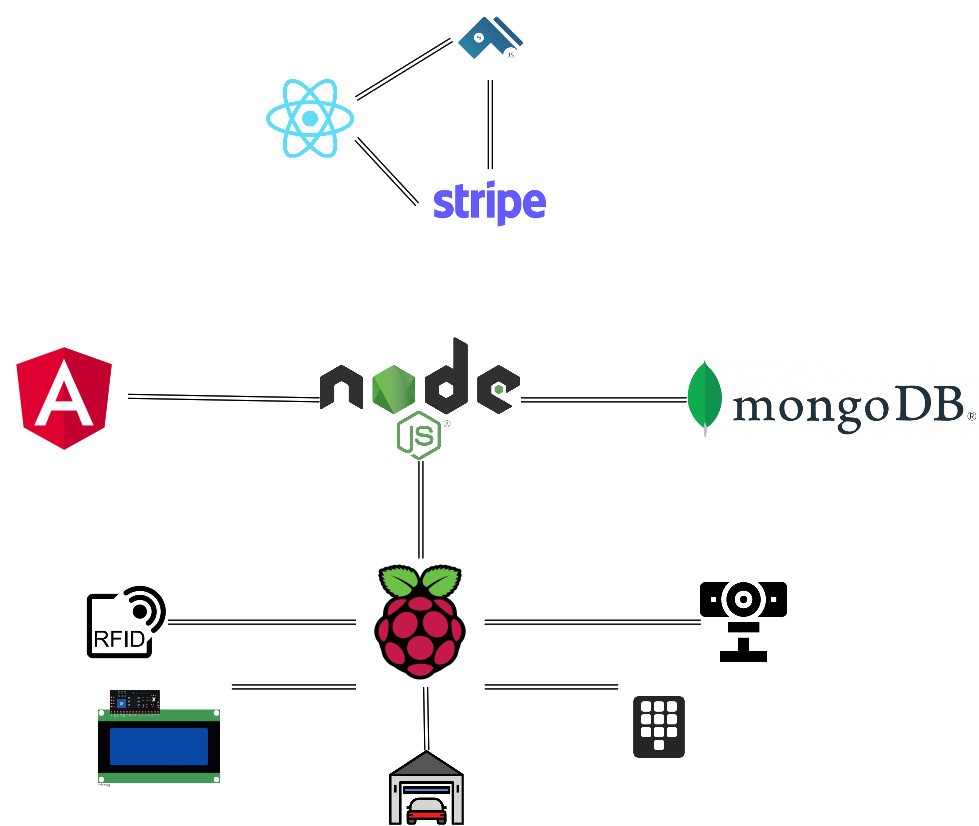
\includegraphics[width=10cm]{pics/APERTASystemarchitektur.jpg}
    \caption{Systemarchitektur}
    \end{figure}
Diese Diplomarbeit setzt sich aus zwei voneinander unabhängigen Systemen zusammen. Das Shopsystem, bestehend aus einem React-Frontend, kommuniziert mit zwei Bibliotheken, CommerceJS und Stripe, welche für die Produktverwaltung, sowie den Bezahlvorgang zuständig sind. Das Angular-Frontend des Dashboard in Verbindung mit dem NodeJS Server, der MongoDB Datenbank sowie dem Raspberry bietet das zweite System.
Der Raspberry ist über GPIOs mit dem RFID-Leser, dem Nummernfeld und dem Display verbunden. Weiters wurde die Kamera an einen der USB 3.0 Ports des Raspberry angeschlossen. Wird eine der Zutrittsmöglichkeiten positiv abgeschlossen, steuert der Raspberry Pi das Relais an, welches die Garage öffnet.
\section{Frontend (Angular-Applikation) [DH]}
\setauthor{David Hauser}

Die Profilseite ist ein wichtiger Teil des webbasierten Clients, jedoch gibt es für die einzelnen Bauteile auch eigene Unterseiten. Auf diesen Seiten hat die Benutzerin oder der Benutzer noch mehr Möglichkeiten über die Komponenten zu entscheiden. Um die Daten für den Raspberry Pi bereitstellen zu können, werden noch weitere Funktionen benötigt.

\subsection{Aufbau von Angular}

\begin{figure}[h]
    \centering
    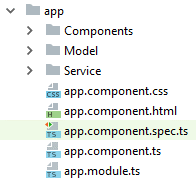
\includegraphics[width=0.4\textwidth]{pics/Aufbau_Angular.png}
    \caption{Aufbau eines Angular Projekts}
    \end{figure}

Die Applikation ist, wie bei Angular-Projekten üblich, in unterschiedliche Ordner aufgeteilt. Der App-Ordner besitzt mehrere Unterordner, welche ähnliche Funktionen gruppieren.

\subsubsection{App}
Die Dateien, welche mit app.component beginnen, werden als App bezeichnet. Sie stellen die Hauptkomponente der Angular-Applikation dar. Für das Routing im Projekt könnte noch eine app-routing.module.ts Datei angelegt werden. Wird diese nicht erstellt, kann das Routing auch in der app.module.ts durchgeführt werden. 

\begin{lstlisting}[language=typescript, caption=app.module.ts]
    @NgModule({
  declarations: [
    AppComponent,
    ProfileComponent,
    NfcSettingsComponent,
    KeyPadSettingsComponent,
    SignSettingsComponent,
    LoginComponent,
    NavbarComponent,
    KeypadComponent,
    SignComponent
  ],
  imports: [
    BrowserModule,
    BrowserAnimationsModule,
    [RouterModule.forRoot(routes)],
    MatCardModule,
    ReactiveFormsModule,
    MatFormFieldModule,
    MatInputModule,
    MatButtonModule,
    MatSelectModule,
    MatRadioModule,
    MatIconModule,
    HttpClientModule
  ],
  providers: [],
  exports: [RouterModule],
  bootstrap: [AppComponent]
})
export class AppModule { }
\end{lstlisting}

In dieser Datei finden die Imports der Node-Module statt. Zusätzlich werden auch die verwendeten Services importiert. Die Module werden unterteilt, um sie strukturierter zu speichern. Außerdem werden die Angular Materials Module importiert, welche der Programmiererin oder dem Programmierer helfen, die Applikation leichter zu gestalten. 

\begin{lstlisting}[language=typescript, caption=Routing der Komponenten in der app.module.ts]
const routes: Routes = [
  { path: '', component: LoginComponent },
  { path: 'profile', component: ProfileComponent },
  { path: 'nfcSettings', component: NfcSettingsComponent},
  { path: 'keyPadSettings', component: KeyPadSettingsComponent},
  { path: 'signSettings', component: SignSettingsComponent},
  { path: 'addSign', component: AddSignComponent },
  { path: 'login', component: LoginComponent},
  { path: 'nav', component: NavbarComponent}
];
\end{lstlisting}

Mittels [RouterModule.forRoot(routes)] werden die Routen innerhalb des Projekts definiert. Sie navigieren die Userin oder der User durch die einzelnen Views.

Um den Pfad einer Route zu bestimmen wird der Pfadname angegeben.  Darauf folgt die Komponente, welche aufgerufen werden soll. 

\begin{lstlisting}[caption=app.component.html]
    <app-navbar></app-navbar>
    <router-outlet></router-outlet>    
\end{lstlisting}

Diese html-Datei ist der Kern der Anwendung. Mittels <app-navbar> wird die Navbar eingebunden, welche dauerhaft am Client angezeigt wird. Im Befehl <router-outlet> werden die Komponenten, die bei den Routen im app.module.ts angegeben sind, angezeigt.

\subsubsection{Komponenten}
In diesem Ordner sind alle Komponenten auffindbar, die in der Anwendung verwendet werden. Es sind also alle Seiten mit ihren Unterkomponenten, wobei eine Seite eine gesamte Komponente darstellt, zu finden.

\subsubsection{Service}
Dieser Ordner beinhaltet alle Dienste für die Applikation. Die Funktionsweise und Verwendung wird nachfolgend noch genauer beschrieben.

\subsection{Angular-Komponente}
Die Anzeigeelemente in Angular werden als Komponenten bezeichnet. Diese werden als eigene HTML-Elemente definiert. Sie stellen abhängig von ihrer Anzeige-Logik und den Daten den Zustand der Anwendung dar.

\begin{figure}[h]
    \centering
    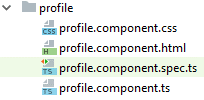
\includegraphics[width=0.4\textwidth]{pics/Aufbau_Komponente.png}
    \caption{Aufbau einer Angular Komponente}
\end{figure}

Jede Komponente besteht aus:

\begin{itemize}
    \item HTML
    \item CSS
    \item TypeScript
    \item spec.TypeScript 
\end{itemize}

Wie sich die Komponente verhält und welche Daten sie anzeigt, wird in der TypeScript Klasse definiert. Ihr Aussehen und wo die Daten genau angezeigt werden sollen, wird in der HTML-Datei festgelegt. Ihr Design kann über das CSS-File bestimmt und beeinflusst werden.
\cite{AngularKomponenten}

\subsection{Services}
Für die Daten und Logik, welche nicht nur in einer Komponente verwendet werden, werden Angular Services genutzt. Darin werden Attribute und Methoden definiert, welche anschließend von anderen Komponenten und Services verwendet werden können.

\begin{figure}[h]
    \centering
    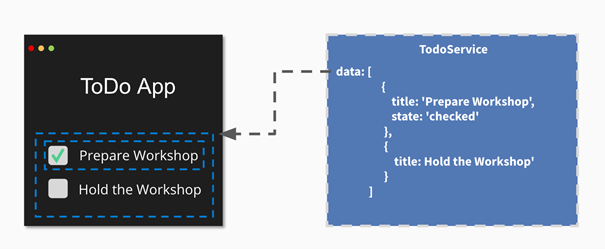
\includegraphics[width=0.8\textwidth]{pics/Service_Klasse.png}
    \caption{Auslagern einer Service Klasse}
    \cite{Service}
\end{figure}

Das Service liefert also die eigentlichen Daten für die Komponente. Die Daten gehören nicht in die Komponente. Explizite Aufgaben sollten in einem entsprechenden Service ausgelagert werden. Um die ausgelagerten Daten dann in die Komponente zu bekommen, wird Dependency Injection verwendet.

\subsection{Dependency Injection}
Unter Dependency Injection oder auch Inversion of Control wird ein Design-Pattern verstanden. Die Dependency sollte also nicht von der aufrufenden Stelle selbst erzeugt werden. Letztere sollte die Kontrolle abgeben und nur die Abhängigkeiten definieren. 

\begin{figure}
  \centering
  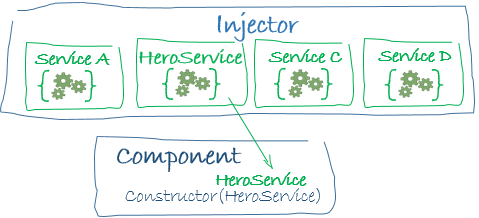
\includegraphics[width=0.6\textwidth]{./pics/DependencyInjection.png}
  \caption{Dependency Injection}
\end{figure}
\pagebreak
In Angular werden die verschiedenen Services vom sogenannten Injector verwaltet. Dieser gibt eine Referenz des Service und die aufrufende Stelle an, sofern dieser definiert ist. Über den Konstruktor wird die Definition der Abhängigkeit abgebildet. In einem Konstruktor können dann die Methoden des Service aufgerufen und somit auf die Daten zugegriffen werden.
\cite{AngularService}

\section{Frontend (React-Applikation) [BG]}
\setauthor{Benjamin Golic}
Die React-Applikation besteht aus mehreren Komponenten.

\subsubsection{Applikationsstruktur}
\setauthor{Benjamin Golic}

\begin{figure}[H]
  \centering
  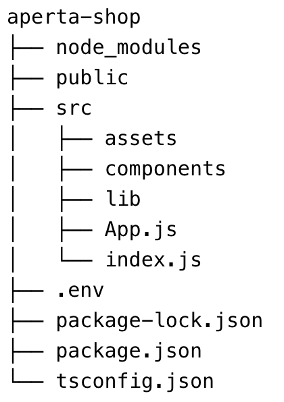
\includegraphics[width=0.5\textwidth]{pics/react-ordnerstruktur.png}
  \caption{Ordnerstruktur der React-Applikation}
\end{figure}

Grundsätzlich besteht eine React-App aus Node-Modules, einer TS-Config, einem Package-File und dem Source-Code. Das Package-File dient zur Verwaltung der Projekt-Abhängigkeiten und -Metadaten. Die TS-Config ist für die Kompilieroptionen des Projekts verantwortlich.

Des Weiteren verwenden Entwicklerinnen oder Entwickler eine „.env“-Datei in ihren Projekten. Da diese Datei sensible Daten, wie beispielsweise API-Schlüssel enthalten, werden sie nicht versioniert. Aus diesem Grund müssen die Entwickelnden die Datei lokal gespeichert haben. Die „.env“-Datei ist eine gewöhnliche Textdatei, die Umgebungsvariablen beinhaltet.
\cite{envFile}

\begin{figure}[H]
  \centering
  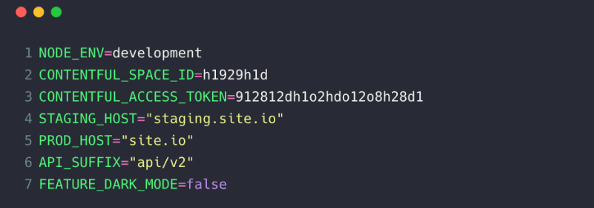
\includegraphics[width=0.8\textwidth]{pics/bsp-env.png}
  \caption{Ordnerstruktur der React-Applikation}
  \cite{envExample}
\end{figure}

\subsubsection{React-Komponente [BG]}
\setauthor{Benjamin Golic}

\begin{figure}[H]
  \centering
  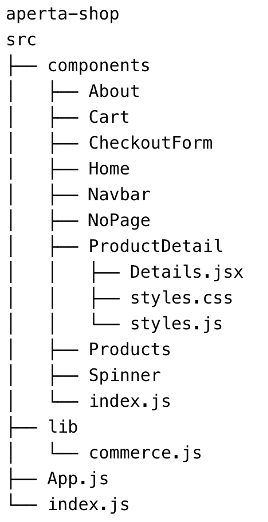
\includegraphics[width=0.3\textwidth]{pics/react-komponentenstruktur.png}
  \caption{Komponenten der React-Applikation und Aufbau der „ProductDetail“-Komponente}
\end{figure}

Grundsätzlich gibt es keine Vorgaben wie eine React-Komponente aufgebaut sein soll. Es gibt lediglich gängige Ansätze, an die sich die Entwickelnden halten können. Die zwei beliebtesten Ansätze sind die Gruppierung nach Markmalen oder Routen und die Gruppierung nach dem Dateitypen.
\cite{reactComponents}

In diesem Projekt bestehen die Komponenten aus einer „.jsx“-Datei, einer „styles.js“-Datei und meistens zusätzlich aus einer „styles.css“-Datei. Die „.jsx“-Datei ist für den Aufbau und der Logik verantwortlich. Die anderen beiden Dateien werden für die Gestaltung verwendet.

Die „App.js“-Datei ist die Haupt-Komponente der React-Applikation. Diese Komponente dient als Container für alle anderen Komponenten. Sie enthält unter anderem das Routing.
\cite{appJS}

Das Routing dient dazu, die Benutzeroberfläche mit dem URL zu synchronisieren. Es legt fest, welcher Inhalt bei welcher URL angezeigt werden soll. Es ermöglicht die Navigierung durch die Web-Applikation, ohne die komplette Seite neu laden zu müssen. 
\cite{reactRouting}

\begin{lstlisting}[language=JavaScript, caption=Source-Code des Routers, label=lst:impl:reactRouterSourceCode]
  <Router>
    <div style={{ display: 'flex' }}>
      <CssBaseline />
      <Navbar totalItems={cart.total_items} handleDrawerToggle={handleDrawerToggle} />
      <Routes>
        <Route path="/components" element={<Products products={products} onAddToCart={handleAddToCart} handleUpdateCartQty />} />
        <Route path="/packages" element={<Products products={pproducts} onAddToCart={handleAddToCart} handleUpdateCartQty />} />
        <Route path="/home" element={<Home products={pproducts} onAddToCart={handleAddToCart} handleUpdateCartQty/>} />
        <Route path="/about" element={<About />} />
        <Route path="/cart" element={<Cart cart={cart} onUpdateCartQty={handleUpdateCartQty} onRemoveFromCart={handleRemoveFromCart} onEmptyCart={handleEmptyCart} /> } />
        <Route exact path="/checkout" element={ <Checkout cart={cart} order={order} onCaptureCheckout={handleCaptureCheckout} error={errorMessage} /> } />
        <Route exact path="/" element={<Home products={pproducts} onAddToCart={handleAddToCart} handleUpdateCartQty/>} />
        <Route exact path="/detail/:id" element={<Details onAddToCart={handleAddToCart} handleUpdateCartQty />} />
        <Route path="*" element={<NoPage />} />
      </Routes>
    </div>
  </Router> 
\end{lstlisting}

\subsubsection{Gestaltung der Benutzeroberfläche}
\setauthor{Benjamin Golic}

Für die Gestaltung der Benutzeroberfläche kamen CSS und JSS zum Einsatz.

JSS ist eine JavaScript-Library, die es Entwickelnden ermöglicht, Stile auf konfliktfreie und wiederverwendbare Weise zu schreiben. Diese Bibliothek kann sowohl client- als auch serverseitig kompiliert werden. 
\cite{jss}

\begin{lstlisting}[language=JavaScript, caption=Beispiel Source-Code für die Verwendung von JSS, label=lst:impl:bspJSS]
  import jss from "jss";
  import preset from "jss-preset-default";
  
  jss.setup(preset());
  
  const styles = {
    wrapper: {
      padding: 40,
      background: "#f7df1e",
      textAlign: "center"
    },
    title: {
      font: {
        size: 40,
        weight: 900
      },
      color: "#24292e"
    },
    link: {
      color: "#24292e",
      "&:hover": {
        opacity: 0.5
      }
    }
  };
\end{lstlisting} \cite{jssExample}

Da Webapplikationen auch auf mobilen Geräten verfügbar sein sollen, muss die Benutzeroberfläche an unterschiedlichste Bildschirmgrößen angepasst werden. Hierbei wird von „Responsive Design“ gesprochen. Um dies zu realisieren, können Entwicklerinnen oder Entwickler auf bestimmte CSS-Libraries zurückgreifen. Allerdings bietet klassisches CSS „Flexbox“ und „Grid“ Möglichkeiten für die Realisierung eines Responsive Designs. Bei diesen Möglichkeiten handelt es sich um zwei signifikant unterschiedliche Layout-Technologien.

\subsubsection{CSS-Flexbox}
\setauthor{Benjamin Golic}

Dieses Modell bietet sich besonders für lineare Strukturen an, da es mit zwei Achsen, auf denen Inhalte verteilt werden können, arbeitet. Grundsätzlich wird hier mit einem Flex-Container und den darin enthaltenen Kind-Elementen (Flex-Items) gearbeitet. 
\cite{flexbox}

\begin{figure}[H]
  \centering
  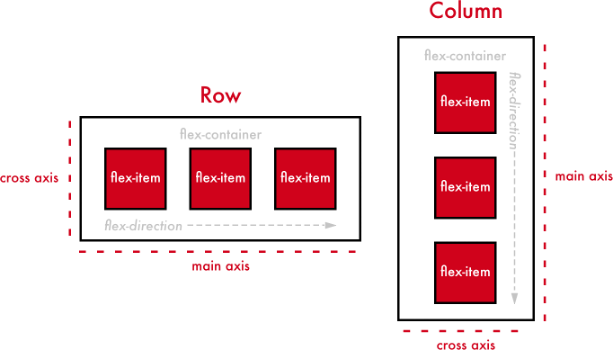
\includegraphics[width=0.8\textwidth]{pics/flexDirection.png}
  \caption{Darstellung der Flex-Direction}
  \cite{flexbox2}
\end{figure}


\begin{lstlisting}[language=HTML, caption=HTML-Code vom Aufbau einer Flexbox , label=lst:impl:flexHTML]
  <div class="flex-container">
    <div class="flex-item"></div>
    <div class="flex-item"></div>
    <div class="flex-item"></div>
    <div class="flex-item"></div>
  </div>
\end{lstlisting} \cite{flexbox}

Um die Flexbox auf dem Container-Element zu aktivieren, muss dem „flex-container“ im CSS-Code die Eigenschaft „display:flex“ zugewiesen werden. 
\cite{flexbox}

\begin{lstlisting}[language=CSS, caption=CSS-Code zur Aktivierung der Flexbox, label=lst:impl:flexCSS]
  .flex-container {
    display: flex;
  }
\end{lstlisting} \cite{flexbox}

\subsubsection{CSS-Grid}
\setauthor{Benjamin Golic}

Mit diesem Modell werden Zeilen und Spalten für einen Bereich definiert, für welche dann Elemente zugewiesen werden. Grundsätzlich wird hier mit einem Elternelement gearbeitet, in dem das Raster definiert wird. Die darin enthaltenen Kind-Elemente werden im Raster positioniert. 
\cite{cssgrid}

\newpage

\begin{lstlisting}[language=HTML, caption=HTML-Code vom Aufbau eines Grids, label=lst:impl:gridHTML]
  <div class="container"> 
    <div>Element 1</div> 
    <div>Element 2</div> 
    <div>Element 11</div> 
    <div>Element 12</div> 
 </div>
\end{lstlisting} \cite{cssgrid}

Dem Elternelement wird mit Hilfe der CSS-Eigenschaft „display:grid“ mitgeteilt, dass CSS-Grids verwendet werden. 

\begin{lstlisting}[language=CSS, caption=CSS-Code zur Aktivierung des Grids, label=lst:impl:gridCSS]
.container { 
  display: grid; 
  grid-template-rows:200px 1fr 100px; 
  grid-template-columns:25% 25% 25% 25%; 
}
\end{lstlisting} \cite{cssgrid}

Mit den Eigenschaften „grid-template-columns“ und „grid-template-rows“ werden Rasterlinien festgelegt.
\cite{cssgrid}

\begin{figure}[H]
  \centering
  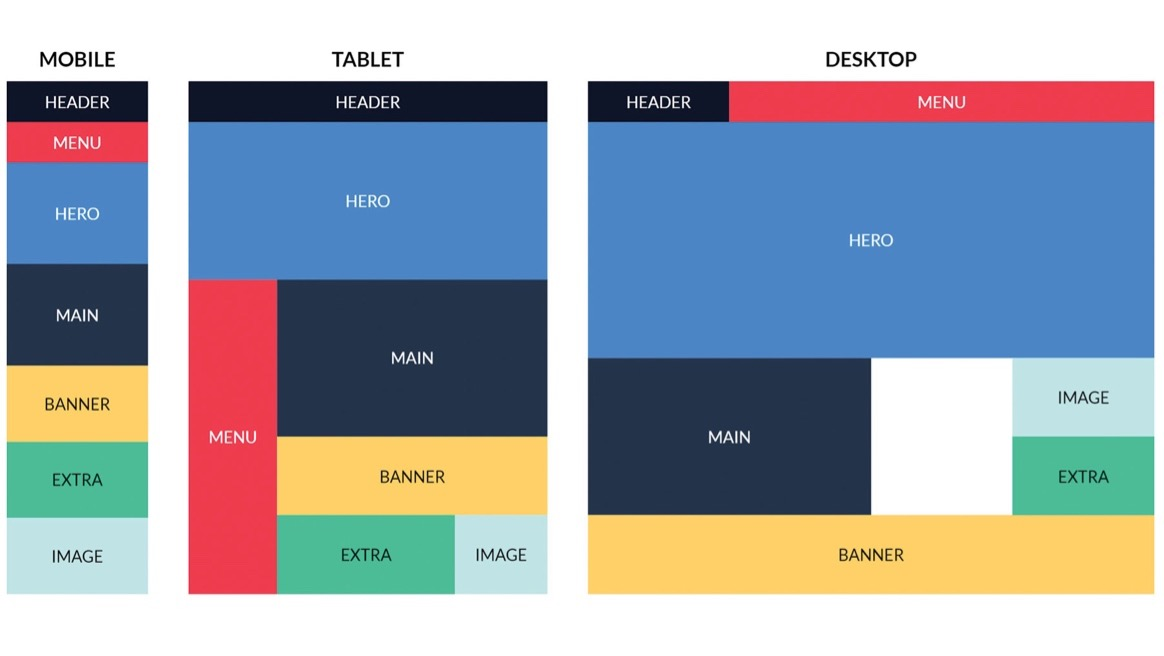
\includegraphics[width=0.9\textwidth]{pics/cssGridDarstellung.jpg}
  \caption{Darstellung eines Responsive-Designs durch CSS-Grids}
  \cite{cssgridDarstellung}
\end{figure}

\newpage

\subsubsection{Commerce.js}
\setauthor{Benjamin Golic}

Commerce.js ist ein Headless-E-Commerce-Backend, welches die Integration von E-Commerce in jedes Web- und Mobil-Projekt beschleunigt. Die JavaScript-SDK und API-Suite wurden mit Fokus auf Entwickelnde entwickelt. Außerdem ermöglicht es Entwickelnden, dasselbe E-Commerce-Backend für eine Web-App und einer mobilen Anwendung zu verwenden.
\cite{commerceJS}\\

Mit Commerce.js ist es möglich eigene Produkte mit beliebigen Produktinformationen hinzuzufügen.

\begin{figure}[H]
  \centering
  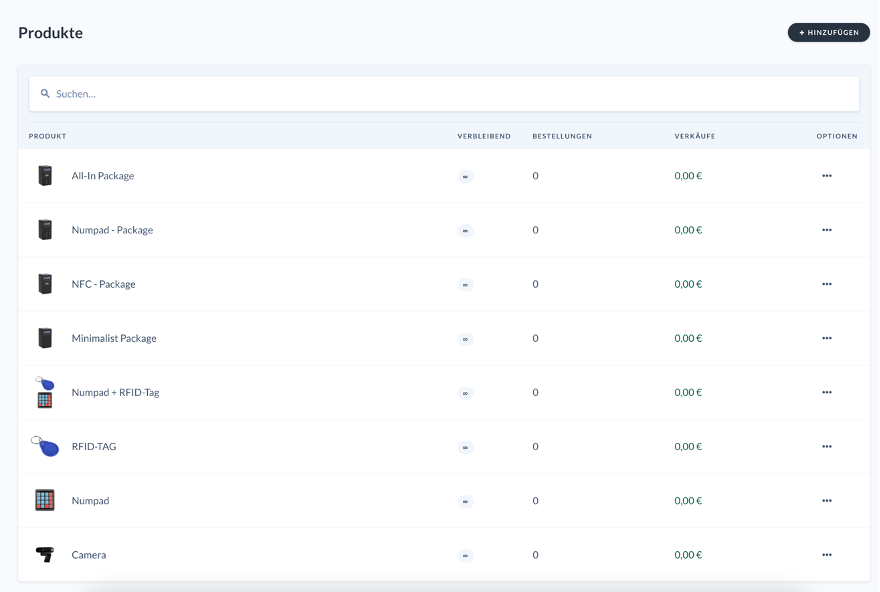
\includegraphics[width=0.9\textwidth]{pics/apertaProdukteCommerce.png}
  \caption{APERTA-Produkte in Commerce.js}
\end{figure}

Da die Nutzung des Verwaltungs-Dashboards keinen Programm-Code erfordert, ermöglicht es Content-Autoren, Fulfillment-Teams und Geschäftsinhabern die Verwaltung von Produkten, Kunden und Bestellungen.
\cite{commerceJS}

\newpage

\subsubsection{Stripe}
\setauthor{Benjamin Golic}

Stripe ist eine Online-Zahlungsabwicklungs- und Kreditkartenverarbeitungsplattform für Unternehmen. Diese Plattform ermöglicht eine sichere und effiziente Verarbeitung von Geldern per Kreditkarte oder Bank und überweist diese Gelder auf das Konto des Verkaufenden. Stripe umfasst sowohl eine Plattform für die Zahlungsabwicklung als auch ein Gateway für Kreditkartenzahlungen. Zusätzlich zu einmaligen Bezahlvorgängen bietet Stripe auch die Möglichkeit für Abonnements.

Bei einer korrekten Integration werden die vom Kaufenden eingetragenen Informationen beim Bezahlungsvorgang vom Web-Shop über die Stripe-Software gesendet. Diese überprüft, ob das zu zahlende Geld verfügbar ist und verarbeitet die Zahlung, bevor sie an das Händlerkonto gesendet wird. Nach einem erfolgreichem Zahlungsprozess erhalten Kaufende und Verkaufende eine Verkaufsbestätigung.

Falls bei einem Zahlungsvorgang etwas schieflaufen sollte, beispielsweise durch unzureichende Deckung auf dem Konto des Kaufenden, wird die Transaktion durch Stripe abgelehnt. Des Weiteren wird der Kaufende darüber benachrichtigt und bekommt die Möglichkeit, eine andere Zahlungsmethode zu verwenden.

Darüber hinaus überwacht Stripe auch betrügerische Transaktionen und blockiert alle verdächtig erscheinenden Transaktionen.

Bei Stripe ist man nicht auf eine Zahlungsart beschränkt. Es gibt eine große Auswahlmöglichkeit an viele gängigen Bezahlungsmethoden. Außerdem kann man mehrere davon aktivieren.

Des Weiteren liefert Stripe den Verkaufenden jede Menge an Statistiken und Berichten über die getätigten Verkäufe.

\cite{stripe}

\begin{figure}[H]
  \centering
  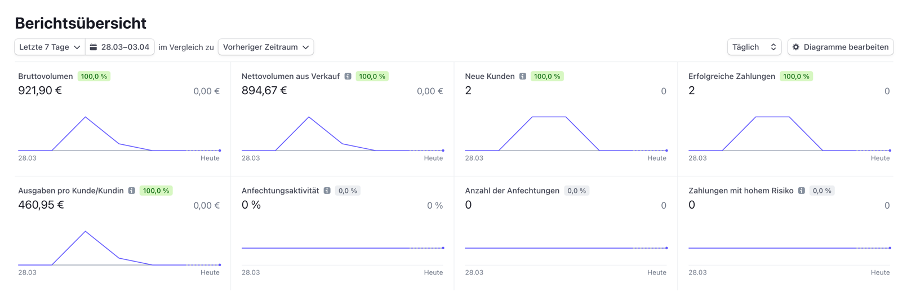
\includegraphics[width=0.9\textwidth]{pics/StripeBericht.png}
  \caption{Stripe-Berichtsübersicht}
\end{figure}

\begin{spacing}{1}
\chapter{Umsetzung}\label{chapter:implementation}
\end{spacing}
\section{Implementierung des Backend [SK]}
\setauthor{Simon Koll}
Das Backend besteht aus einer JavaScript Datei, in welcher sämtliche Endpunkte definiert werden. Weiters benötigt das Backend einige Pakete, um beispielsweise mit der Datenbank zu kommunizieren. Diese werden in \verb|package.json| aufgeführt. Bei erstmaliger Installation wird die Datei automatisch durchlaufen, und installiert alle benötigten Dateien und Pakete. Dazu wird der Terminal-Befehl \verb|npm install| ausgeführt. Der Node Package Manager installiert alle Pakete im Ordner \verb|node_modules|.\\
Der Server selbst wird weiters eingeteilt in:

\begin{itemize}
    \item \textit{Imports: } Zu Beginn werden alle benötigten Pakete, wie unter anderem \textbf{express} importiert. Dies geschieht mittels \verb|require('express')|.
    \item \textit{Setup:  } In weiterer Folge werden benötigte Variablen, wie die Verbindungs-URL der MongoDB Datenbank, definiert. Da die Datenbank und der Server auf der selben Maschine laufen, wird der Host auf \verb|mongodb://127.0.0.1:27017| gesetzt. Der weitere Aufbau der UTL besteht aus Parametern wie zum Beispiel der \verb|serverSelectionTimeOutMS|.
    \item \textit{Express: }  Es bietet Möglichkeiten zum schreiben von Handlern für Anfragen mit verschiedenen HTTP-Verben an verschiedenen URL-Pfaden (Routen) sowie zur Festlegung allgemeiner Einstellungen für Webanwendungen, wie z. B. des Ports, der für die Verbindung verwendet werden soll, und des Speicherorts von Vorlagen, die für das Rendering der Antwort verwendet werden. Um die Express-Applikation zu erstellen, wird \verb|const app = express();| verwendet.
    \item \textit{Header: } Um den Zugriff des Raspberry auf den Server zu gewährleisten, müssen die Header-Parameter gesetzt werden. Dies geschieht mittels \verb|app.use()| und einer als Parameter übergebenen Funktion, in der mit \verb|res.setHeader()| die Header-Parameter gesetzt werden. Diese bestimmen welche IP-Adressen auf den Server zugreifen können, welche Methoden verwendet werden dürfen, sowie die zugelassenen Header bei Anfragen des Clients.
    \item \textit{Konfiguration der Datenbank-Verbindung: } Um den Server mit der Datenbank kommunizieren zu lassen, sind einige Parameter notwendig. Diese werden wie folgt gesetzt: 
    \begin{lstlisting}[language=Python, caption=Konfiguration der Datenbankanbindung, label=lst:impl:dbconf]
    MongoClient.connect(connstring, {useUnifiedTopology: true})
    .then(client => {
        const db = client.db('aperta')

        const licenseplateCollection =
        db.collection('licenseplate')
        const rfidCollection = db.collection('rfid')
        const numpadCollection = db.collection('numpad')
    \end{lstlisting}
    \item \textit{Handler: } Handler sind die Endpunkte, mit denen die Clients kommunizieren. Diese unterscheiden sich je nach Art der Anfrage. Die Anfragen werden mittels \verb|app.get()|, \verb|app.post()|, \verb|app.put()| und \verb|app.delete()| definiert. Als Parameter wird der Endpunkt angegeben, sowie die Funktion, welche ausgeführt wird, wenn der Endpunkt aufgerufen wird. Eine Abfrage der Kennzeichen, welche in der Datenbank gespeichert sind, sieht somit wie folgt aus: 
    \begin{lstlisting}[language=JavaScript, caption=Abfrage der Kennzeichen, label=lst:impl:getlicenseplates]

        app.get('/get-licenseplates', function(req, res) {
            licenseplateCollection.find().toArray()
                .then(results => {
                    console.log("retrieving licenseplates")
                    res.send(results)
                })
                .catch(error => console.error(error))
                // do something here
        })
    \end{lstlisting}
    \item \textit{Verbindung:} Die Funktion \verb|app.listen()| wird verwendet, um die Verbindungen an den angegebenen Host und Port zu binden und abzuhören. Diese Methode ist identisch mit der Methode \verb|http.Server.listen()| von Node.
    Wenn die Portnummer weggelassen wird oder 0 ist, weist das Betriebssystem einen beliebigen unbenutzten Port zu, was für Fälle wie automatisierte Aufgaben (Tests usw.) nützlich ist.
    Die von express() zurückgegebene App ist in Wirklichkeit eine JavaScript-Funktion, die als Callback an die HTTP-Server von Node übergeben wird, um Anfragen zu bearbeiten.
    \end{itemize}
\section{Implementierung der Kennzeichenerkennung[SK]}
\setauthor{Simon Koll}
\subsection{Funktionsweise}
Wie bereits in Kapitel \ref{lsg:def:anpr} angeführt, besteht die Kennzeichenerkennung aus 3 Schritten. Bevor diese jedoch durchlaufen werden können, müssen zuerst alle notwendigen Bibliotheken installiert und importiert werden. Diese können mittels \verb|pip3 install <name>|, oder aber auch mit \verb|sudo apt-get install <name>| installiert werden. \\
Nachdem alle Bibliotheken und das Modul zur Überprüfung des Kennzeichens importiert wurden, beginnt mit \verb|cap = cv2.VideoCapture(0)| das Aufzeichnen des Bildes. Dieses wird durch eine Schleife ausgeführt, bis das Programm beendet wird. Falls die Kamera nicht aufgenommen werden kann, wird eine Fehlermeldung ausgegeben.
\subsubsection{Graustufenbild}
Nachdem das Bild angezeigt wurde, wird der erste Filter angewendet. Dabei handelt es sich um einen Filter, welcher das Bild in ein Graustufenbild umwandelt. Dieser wird  mit der Methode \verb|cv2.cvtColor(img, cv2.COLOR_BGR2GRAY)| aufgerufen.
\begin{figure}[H]
\centering
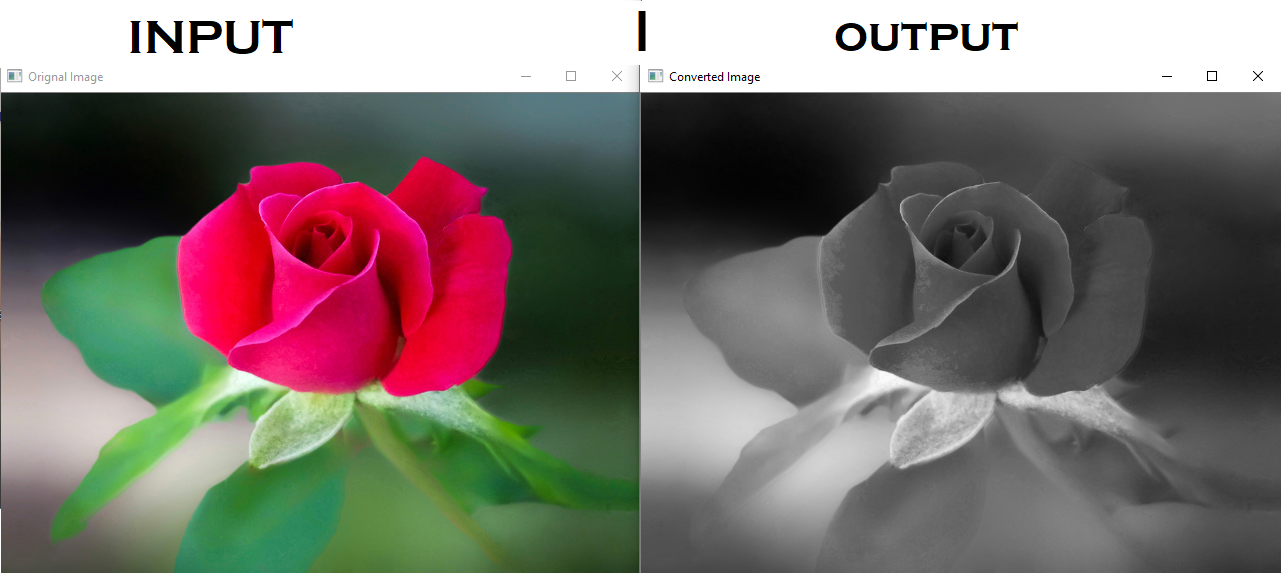
\includegraphics[width=0.8\textwidth]{pics/Color2Gray.PNG}
\caption{Aufgenommenes Bild vs. Graustufenbild}
\cite{grayscaleImage}
\label{fig:anpr_1}
\end{figure}

\subsubsection{Filter}
Als zweiter Filter fungiert ein \verb|cv2.bilateralFilter|. Die wichtigste Eigenschaft der bilateralen Filterung ist, dass sie keine Mittelwertbildung über die Kanten vornimmt. Deshalb wird sie auch als kantenerhaltender Filter bezeichnet. Bevor  die mathematischen Grundlagen des Bilateralfilters erklärt werden, ist es jedoch sinnvoll, kurz auf die Gaußsche Filterung einzugehen, da diese dem bilateralen Filter ähnlich ist.
Die Gaußsche Filterung ist ein gewichteter Durchschnitt der Intensität der benachbarten Positionen, wobei die Gewichtung mit dem räumlichen Abstand zur mittleren Position abnimmt.

Mathematisch gesehen ist ein mit Gaußscher Unschärfe gefiltertes Bild gegeben durch:
\begin{figure}[H]
    \centering
    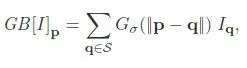
\includegraphics[width=0.5\textwidth]{pics/GBFilteredPic.jpeg}
    \caption{Ein mit Gaußscher Unschärfe gefiltertes Bild}
    \cite{GBfilteredPicture}
    \label{fig:anpr_2}
    \end{figure}
Dabei sind \textit{p} und \textit{q} die Position der Pixel, I kennzeichnet das Bild und G\(\sigma\)(x) den sogenannten zweidimensionalen Gauß-Kernel. 
\begin{figure}[H]
    \centering
    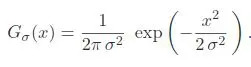
\includegraphics[width=0.5\textwidth]{pics/Gaussian-Filter-Formula-2.jpeg}
    \caption{Gauß-Kernel}
    \cite{GBfilteredPicture2}
    \label{fig:anpr_3}
    \end{figure}
    G\(\sigma\) ist ein räumlicher Gauß, der den Einfluss der entfernten Pixel verringert. Der Abstand zwischen den Pixeln wird mit \(G\sigma(\|p-q\|)\) angegeben. Hierbei ist \(\sigma\) die Ausdehnung der Nachbarschaft.\\
    Der Gaußsche-Unschärfefilter untersucht nur naheliegende Pixel bei der Filterung. Es wird nicht berücksichtig, ob die Pixel die selbe Intensität haben, oder ob die Pixel am Rand liegen oder nicht. Daher werden auch Kanten verwischt, was zu einem Verlust wichtiger Details führt. Die bilaterale Filterung verwendet ebenfalls einen Gauß-Filter im Raum, berücksichtigt aber zusätzlich einen weiteren Gauß-Filter welcher eine Funktion der Pixeldifferenz ist. Die Gaußsche Funktion des Raums sorgt dafür, dass nur nahe gelegene Pixel für die Unschärfe berücksichtigt werden, während die Gaußsche Funktion der Intensitätsdifferenz dafür sorgt, dass nur die Pixel mit ähnlichen Intensitäten wie das zentrale Pixel für die Unschärfe berücksichtigt werden. So bleiben die Kanten erhalten, da die Pixel an den Kanten große Intensitätsunterschiede aufweisen.
    Der wichtige Punkt, der bei der bilateralen Filterung berücksichtigt wird, ist, dass zwei Pixel nicht nur dann nahe beieinander liegen, wenn sie dies räumlich tun, sondern auch, wenn sie eine gewisse Ähnlichkeit im photometrischen Bereich aufweisen. Diese Eigenschaften der bilateralen Filterung überwinden den Nachteil anderer Techniken wie \textit{Averaging Blur} oder \textit{Gaussian Blur}, da sie in der Lage ist, Kanten zu erhalten.\\
    Der Bilaterale Filter wird wie folgt berechnet:
    \begin{figure}[H]
        \centering
        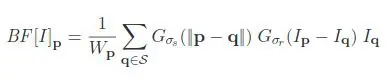
\includegraphics[width=0.5\textwidth]{pics/Bilateral-Filtering-in-Python-OpenCV.jpeg}
        \caption{Bilaterale Filterung Formel}
        \cite{BilateralFormula1}
        \label{fig:anpr:bilat:1}
        \end{figure}
W ist ein Normalisierungsfaktor, welcher mit folgender Formel berechnet wird:
\begin{figure}[H]
    \centering
    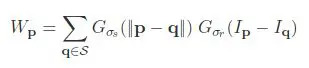
\includegraphics[width=0.5\textwidth]{pics/Bilateral-Filtering-in-Python-OpenCV-Formula2.jpeg}
    \caption{Formel des Normalisierungsfaktors Wp}
    \cite{BilateralFormula2}
    \label{fig:anpr:bilat:2}
    \end{figure}
Dem Gaußschen Filter werden 2 neue Terme hinzugefügt, um den bilateralen Filter zu erhalten. Diese Terme sind:
 \begin{figure}[H]
    \centering
    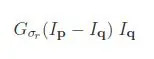
\includegraphics[width=0.3\textwidth]{pics/Bilateral-Filtering-in-Python-OpenCV-Formula3.jpeg}
    \caption{Term 1}
    \cite{BilateralFormula3}
    \label{fig:anpr:bilat:3}
    \end{figure}
\begin{figure}[H]
        \centering
        
\includegraphics[width=0.3\textwidth]{pics/Bilateral-Filtering-in-Python-OpenCV-Formula4.jpeg}
        \caption{Term 2}
        \cite{BilateralFormula4}
        \label{fig:anpr:bilat:4}
        \end{figure}
Wie aus der Gauß-Filterung bereits bekannt, ist\textit{G\(\sigma\)s} ein räumlicher Gauß, welcher den Einfluss enfernter Pixel verringert. Der zweite Term ist \textit{G\(\sigma\)r}, ein Bereichs-Gauß, welcher Einflüsse von Pixeln \textit{q} mit anderen Intensitätswerten als \textit{Ip} verringert. Bereich bedeutet n diesem Fall Größen, die sich auf Intensitäten beziehen, wohingegen der Raum die Lage der Pixel beschreibt.\\
\textit{\(\sigma\)s} ist ein Raumparameter, der für die räumliche Ausdehnung der Kernelgröße in der betrachteten Nachbarschaft beschreibt, und \textit{\(\sigma\)r} hingegen ein Entfernungsparameter, welcher die minimale Amplitude einer Kante beschreibt. Zusammen ergeben die Parameter das Ausmaß der Filterung des Bildes \textit{I}.\\
Daraus folgt:
\begin{compactenum}
    \item Jedes Pixel erhält einen Durchschnitt der benachbarten Pixel, mit dem es überschrieben wird.
    \item Jedes benachbarte Pixel wird durch eine räumliche Komponente, die entfernte Pixel bestraft, und eine Bereichskomponente, die Pixel mit unterschiedlicher Intensität bestraft, gewichtet.
    \item Die Kombination der beiden Komponenten stellen sicher, dass nur nahe, ähnliche Pixel zur Berechnung des Ergebnisses berücksichtigt werden.
\end{compactenum}
Die beiden Parameter \textit{\(\sigma\)r} und \textit{\(\sigma\)s} beeinflussen den bilateralen Filter, indem bei Erhöhung des Entfernungsparameter \textit{\(\sigma\)r} das Ergebnis dem einer Gaußschen Unschärfe ähnelt, und die Erhöhung des räumlichen Parameters \textit{\(\sigma\)s} zur Glättung von großen Merkmalen führt. Veranschaulicht kann dies durch folgende Grafik werden:
\begin{figure}[H]
    \centering
    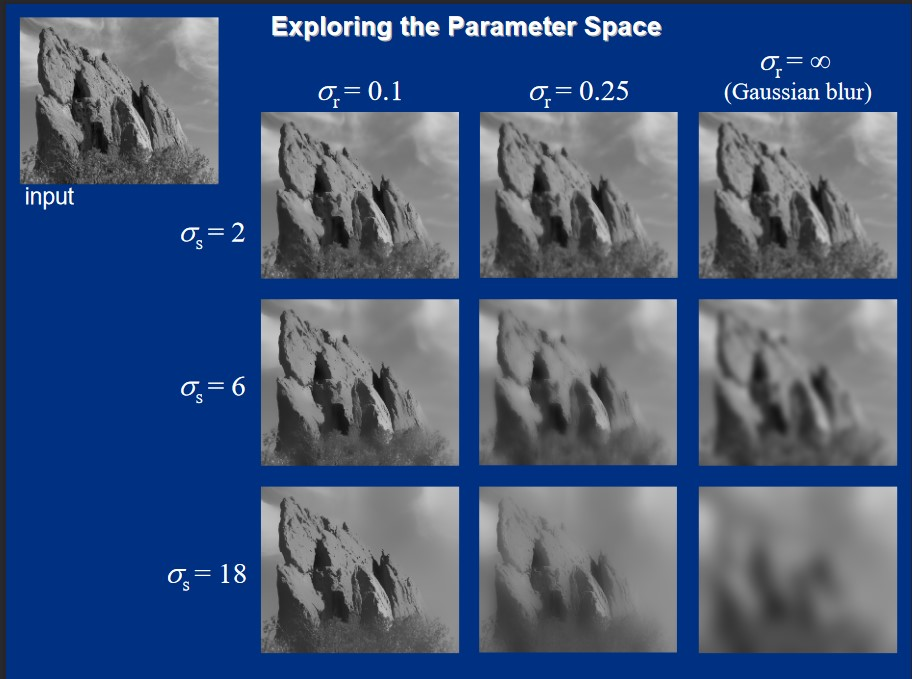
\includegraphics[width=0.5\textwidth]{pics/ParameterBeeinflussungBilateralFilter.jpg}
    \caption{Beeinflussung durch Veränderung der Parameter \textit{\(\sigma\)s} und \textit{\(\sigma\)r}}
    \cite{ParameterBilat}
    \label{fig:anpr:bilat:parameter}
    \end{figure}


Bei der Verwendung der Funktion \verb|cv2.bilateralFilter()| sind folgende Parameter zu berücksichtigen:
\begin{itemize}
    \item \textit{src: } Ein Bild, auf das die Filterung angewendet wird.
    \item \textit{dst: } Das Ergebnis der Filterung. Das Zielbild hat die selbe Größe und den selben Datentyp wie das Ausgangsbild \verb|src|.
    \item \textit{d: }Durchmesser der Pixel-Nachbarschaften, welche zur Berechnung des Filters verwendet werden. Wird dieser negativ, kann auf eine Berechnung durch \textit{sigmaSpace} zurückgegriffen werden.
    \item \textit{sigmaColor: } Ein größerer Wert des Parameters bedeutet, dass weiter entfernte Farben innerhalb der Pixelnachbarschaft zusammengemischt werden, was zu größeren Bereichen mit annähernd gleicher Farbe führt.
    \item \textit{sigmaSpace: }Ein größerer Wert des Parameters bedeutet, dass weiter entfernte Pixel sich gegenseitig beeinflussen, solange ihre Farben nahe genug beieinander liegen. Wenn \textit{d>0} ist, gibt er die Größe der Nachbarschaft unabhängig von sigmaSpace an. Andernfalls ist d proportional zu sigmaSpace.
    \item \textit{borderType: }Randmodus, der für die Extrapolation von Pixeln außerhalb des Bildes verwendet wird.
\end{itemize}
\cite{Filter}
\subsubsection{Kantenerkennung \label{sec:anpr:kantenerkennung}}
Die Kantenerkennung wird mit dem Aufruf von \verb|cv2.Canny()| durchgeführt. Diese Funktion wurde von John F. Canny entwickelt, und ist ein mehrstufiger Algorithmus, welcher in 4 Stufen aufgeteilt werden kann:
\begin{compactenum}
    \item \textit{Rauschunterdrückung: }
    \begin{compactenum}
        \item Da die Kantenerkennung anfällig für Bildrauschen ist, wird zunächst das Bildrauschen mit einem 5x5-Gauß-Filter entfernt
    \end{compactenum}
    \item \textit{Ermittlung des Intensitätsgradienten des Bildes: }
    \begin{compactenum}
        \item  Das geglättete Bild wird dann mit einem Sobel-Kernel sowohl in horizontaler als auch in vertikaler Richtung gefiltert, um die erste Ableitung in horizontaler Richtung \((Gx)\) und vertikaler Richtung \((Gy)\) zu erhalten. Aus diesen beiden Bildern können wir den Kantengradienten und die Richtung für jedes Pixel wie folgt ermitteln:
        \begin{equation}
            \begin{split}
                \begin{aligned}
                    \text{Kantengradient (G)} &= \sqrt{G^2x+G^2y}\\
                    \text{Winkel (\(\theta\))} &= \tan^{-1}(\frac{Gy}{Gx})
                \end{aligned}
            \end{split}
        \end{equation}
        \item Die Richtung der Steigung ist immer senkrecht zu den Kanten. Sie wird auf einen von vier Winkeln gerundet, welche die vertikale, horizontale und zwei diagonale Richtungen darstellen.
    \end{compactenum}
    \item \textit{Non-Maximum-Suppression: }
    \begin{compactenum}
        \item Nachdem Gradient und Richtung ermittelt wurden, wird das Bild vollständig gescannt, um alle unerwünschten Pixel zu entfernen, die möglicherweise nicht die Kante bilden. Zu diesem Zweck wird bei jedem Pixel geprüft, ob es in dessen Umgebung ein lokales Maximum in der Richtung des Gradienten darstellt.
        \begin{figure}[H]
            \centering
            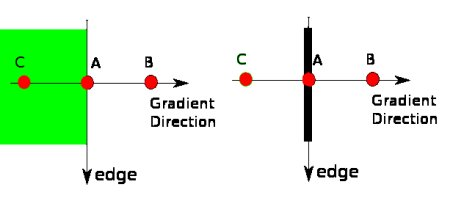
\includegraphics[width=0.5\textwidth]{pics/nms.jpg}
            \caption{Non-Maximum-Suppression}
            \cite{NMSPic}
            \label{fig:anpr:edge:nms}
            \end{figure}
            Punkt A befindet sich auf der Kante in vertikaler Richtung. Die Richtung des Gradienten ist normal zur Kante. Die Punkte B und C liegen in Gradientenrichtung. Punkt A wird also mit den Punkten B und C daraufhin überprüft, ob er ein lokales Maximum bildet. Wenn ja, wird er für die nächste Stufe berücksichtigt, andernfalls wird er unterdrückt (auf Null gesetzt).Das Ergebnis ist ein Binärbild mit dünnen Rändern.
    \end{compactenum}
    \item \textit{Hysterese-Schwellenwertbildung: }
    \begin{compactenum}
        \item  In dieser Phase wird entschieden, welche Kanten wirklich Kanten sind und welche nicht. Hierfür werden zwei Schwellenwerte benötigt, minVal und maxVal. Alle Kanten, deren Intensitätsgradient größer als maxVal ist, sind sicher, dass es sich um Kanten handelt, und diejenigen, die unter minVal liegen, sind sicher, dass es sich um Nicht-Kanten handelt, und werden daher verworfen. Diejenigen, die zwischen diesen beiden Schwellenwerten liegen, werden auf der Grundlage ihrer Konnektivität als Kanten oder Nicht-Kanten klassifiziert. Wenn sie mit "\textit{sure-edge}"-Pixeln verbunden sind, werden sie als Teil von Kanten betrachtet. Andernfalls werden sie ebenfalls verworfen.
        \begin{figure}[H]
            \centering
            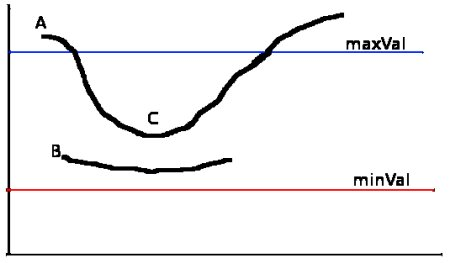
\includegraphics[width=0.5\textwidth]{pics/hysteresis.jpg}
            \caption{Hysterese-Schwellenwertbildung}
            \cite{hysteresisPic}
            \label{fig:anpr:edge:hysteresis}
            \end{figure}
            Die Kante A liegt oberhalb von maxVal, wird also als \"sichere Kante\" betrachtet. Obwohl die Kante C unter maxVal liegt, ist sie mit der Kante A verbunden, so dass sie ebenfalls als gültige Kante betrachtet wird und wir die vollständige Kurve erhalten. Aber die Kante B, obwohl sie oberhalb von minVal liegt und in der gleichen Region wie die Kante C ist, ist nicht mit einer \"sicheren Kante\" verbunden, so dass sie verworfen wird. Es ist also sehr wichtig, dass minVal und maxVal entsprechend ausgewählt werden, um das richtige Ergebnis zu erhalten.
            In dieser Phase werden auch kleine Pixel entfernt, wobei davon ausgegangen wird, dass die Kanten lange Linien sind. Dadurch enstehen starke Kanten im Bild.
    \end{compactenum}
\end{compactenum}
Angewendet auf ein Graustufenbild, sieht das Ergebnis der Kantenerkennung wie folgt aus:
\begin{figure}[H]
    \centering
    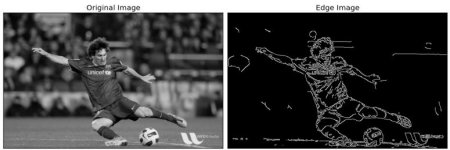
\includegraphics[width=0.8\textwidth]{pics/canny1.jpg}
    \caption{Ergebnis der Kantenerkennung}
    \cite{CannyPic}
    \label{fig:anpr:edge:canny}
    \end{figure}
\subsubsection{Konturenfindung}
Konturen können einfach als eine Kurve erklärt werden, die alle kontinuierlichen Punkte (entlang der Grenze) verbindet, die dieselbe Farbe oder Intensität haben. Die Konturen sind ein nützliches Werkzeug für die Formanalyse und die Erkennung von Objekten.
Mit dem Ergebnis der Kantenerkennung aus \ref{sec:anpr:kantenerkennung} kann OpenCV Konturen eines weißen Objekts vor einem schwarzen Hintergrund finden. Dies geschieht mit dem Aufruf von \verb|cv2.findContours(thresh, cv.RETR_TREE, cv.CHAIN_APPROX_SIMPLE)|. Die Parameter können wie folgt beschrieben werden:
\begin{compactenum}
    \item \textit{thresh}: Das Bild, auf das die Konturen gesucht werden sollen.
    \item \textit{mode}: Der Modus, der zur Konturensuche verwendet wird.
    \item \textit{method}: Die Methode, die zur Konturennäherung verwendet wird.
\end{compactenum}
Als Rückgabewert gibt die Funktion die Konturen und die Hierarchie aus. Die Konturen sind eine Python-Liste mit allen Konturen im Bild. Jede einzelne Kontur ist ein Numpy-Array mit (x,y)-Koordinaten von Grenzpunkten des Objekts.
Der dritte Parameter, die Konturennäherungsmethode, bestimmt, welche Begrenzungspunkte gespeichert werden. Bei \verb|cv2.CHAIN_APPROX_NONE| werden alle Punkte der Kontur gespeichert. Dies ist aber nicht nötig, da nur der Start- und Endpunkt der Linie benötigt werden. Daher ist es sinnvoller, \verb|cv2.CHAIN_APPROX_SIMPLE| zu verwenden, da diese Methode alle überflüssigen Punkte entfernt und die Konturen komprimiert, um so Speicherplatz zu sparen.
In Abbildung \ref{fig:anpr:contour:cam} wird der Unterschied der beiden Methoden erkenntlich gemacht. Anstelle von 734 Punkten bei der Verwendung von \verb|cv2.CHAIN_APPROX_NONE| werden bei \verb|cv2.CHAIN_APPROX_SIMPLE| nur die Start- und Endpunkte der Konturen und damit insgesamt 4 Punkte gespeichert.\cite{drawContours}
\begin{figure}[H]
    \centering
    
\includegraphics[width=0.8\textwidth]{pics/none.jpg}
    \caption{Unterschied von}
    \cite{CAMPic}
    \label{fig:anpr:contour:cam}
    \end{figure}
\subsubsection{Überprüfung der Konturen}
Im nächsten Schritt wird mittels \verb|imutils.grab_contours| überprüft, welche OpenCV Version verwendet wird. Dies unterscheidet sich in der Länge des Kontur-Tupels:
\begin{itemize}
    \item Ist das Tupel 2 Elemente lang, handelt es sich um OpenCV v2.4, v4-beta oder v4-official
    \item Ist das Tupel 3 Elemente lang, handelt es sich um OpenCV v3, v4-pre oder v4-alpha
\end{itemize}
\cite{imutilsGrabContours}\\
Nachdem die Konturen sortiert wurden, wird der Konturumfang mit \verb|cv2.arcLength| berechnet. Danach wird die Kontur unter Verwendung des Douglas-Peucker-Algorithmus mit dem vorher berechneten Konturumfang angepasst. Kommt dieser zu keinem Ergebnis, wird die Kontur verworfen und eine Fehlermeldung ausgegeben.\\
Wurde jedoch eine geschlossene Kontur mit 4 Eckpunkten gefunden, beginnt die Funktion \verb|cv2.drawContours| mit der Zeichnung der Kontur. Die Funktionsparameter sind zum Einen das Bild, auf das die Kontur gezeichnet werden soll, und zum anderen die Kontur. Weitere Parameter, wie Farbe, Dicke und mehr können ebenfalls übergeben werden.
\cite{drawContours}
\subsubsection{Maskieren der relevanten Bildregion \label{sec:anpr:mask}}
Da für den weiteren Ablauf des Programms nur noch die Region, in der sich das Kennzeichen befindet, relevant ist, wird diese maskiert und als neues Bild gespeichert:

\begin{lstlisting}[language=Python, caption=Maskieren der Kennzeichenregion und Abspeichern in neuem Bild, label=lst:impl:anpr:mask]
    mask = np.zeros(gray.shape, np.uint8)
    new_image = cv2.drawContours(mask, [screenCnt], 0, 255, -1,)
    new_image = cv2.bitwise_and(frame, frame, mask=mask)
    (x, y) = np.where(mask == 255)
    (topx, topy) = (np.min(x), np.min(y))
    (bottomx, bottomy) = (np.max(x), np.max(y))
    Cropped = gray[topx:bottomx+1, topy:bottomy+1]
\end{lstlisting}

\subsubsection{Texterkennung \label{sec:anpr:text}}
Aus dem in \ref{sec:anpr:mask} erzeugten Bild kann nun der Text des Kennzeichens gelesen werden. Dies geschieht mit der Funktion :
\begin{lstlisting}[language=Python, caption=Maskieren der Kennzeichenregion und Abspeicher in neuem Bild, label=lst:impl:anpr:text]
    text = pytesseract.image_to_string(Cropped, config='--psm 11')
\end{lstlisting}

Mit \verb|config='--psm 11'| wird die Priorität der Texterkennung auf den Text selbst gesetzt. Da zuvor schon alle irrelevanten Bereiche des Bildes durch Maskieren entfernt wurden, wurde hier diese Priorität verwendet, um die Ergebnisse der Kennzeichenerkennung zu verbessern. \cite{PSM11} \\
Dadurch kann es aber auch zu Problemen kommen, da nun Sonderzeichen erkannt werden, welche nicht auf dem Kennzeichen existieren. Um alle Leerzeichen und Sonderzeichen zu entfernen, wurden mit \verb|re.sub('[^a-zA-Z0-9 \n\.]', '', text)| alle nicht möglichen Zeichen aus dem Text entfernt.


\subsubsection{Überprufung des erkannten Kennzeichens}
Der Text aus \ref{sec:anpr:text} wird mit dem Aufruf des Modules \verb|checkPlate(text_replaced)| an ein Python-Script übergeben, welches für die weitere Überprüfung zuständig ist.

\begin{lstlisting}[language=Python, caption=Abfrage der Kennzeichen aus der Datenbank, label=lst:impl:anpr:check:db]
    print(type(text))
    r = requests.get('http://130.162.215.116/get-licenseplates')
    val = json.loads(r.text)
\end{lstlisting}

Im Code-Abschnitt \ref{lst:impl:anpr:check} wird die Antwort des Servers in ein JSON-Objekt geladen und mit \verb|json.loads| in ein Python-Objekt umgewandelt, welches die Daten der gefundenen Kennzeichen enthält. Da die Formatierung der Kennzeichen aus der Datenbank sich von dem der Ergebnis der Erkennung unterscheiden kann, wird mit \verb|str.maketrans| eine Zuordnungstabelle erstellt, die im späteren Verlauf von der Methode \verb|str.translate| verwendet wird, um die Formatierungsunterschiede zu beseitigen.\\
Kennzeichen können im Dashboard deaktiviert werden und dürfen in diesem Zustand nicht die Garage öffnen. Um dies zu realisieren, wird der Boolean \verb|active| aus der Datenbankabfrage jedes Kennzeichens überprüft. Wenn dieser Boolean auf \verb|False| steht, wird das Kennzeichen nicht weiter überprüft.\\

 \begin{lstlisting}[language=Python, caption=Überprüfung auf Gleichheit der beiden Strings, label=lst:impl:anpr:check]
    if text.replace(" ", "").translate(table) == value["licenseplate"].translate(table).replace(" ", ""):
        print("licenseplate recognized, initiating opening sequence")
        initiateOpeningSequence()
    else:
        print("not recognized, staying closed")
 \end{lstlisting}
 Sind beide Kennzeichen gleich, wird die Methode \verb|initiateOpeningSequence| aufgerufen, welche das Relais ansteuert.
\section{Implementierung des Displays[SK]}
\setauthor{Simon Koll}
Das Display kann mithilfe von drei verschiedenen Methoden unterschiedliche Texte anzeigen. 
\begin{enumerate}
    \item Kombination des Nummernfeldes korrekt
    \begin{compactenum}
        \item Bei korrekter Eingabe des Nummernfeldes wird das Display wie folgt beschrieben:
        \begin{lstlisting}[language=Python, caption=Ausgabe bei korrekter Eingabe der Kombination auf dem Nummernfeld, label=code_display_correct]
        outString = writingString
        lcd.text("Combination:", 1)
        lcd.text(outString, 2)
        \end{lstlisting}
        Nach einer Wartezeit von 5 Sekunden wird das Display geleert und steht für neue Aufgaben zur Verfügung.
    \end{compactenum}
    \item Kombination des Nummernfeldes nicht korrekt
    \begin{compactenum}
        \item Bei inkorrekter Eingabe des Nummernfeldes soll nicht ausgegeben werden, an welcher Stelle der Eingabe sich der Fehler befindet. Daher gibt das Display \verb|Wrong Combination, please try again| aus.
    \end{compactenum}
    \item NFC-Tag nicht korrekt
    \begin{compactenum}
        \item Bei nicht authorisierten NFC-Karten sowie bei fehlerhaften Lesevorgängen muss das Garagentor verschlossen bleiben. Daher wird in diesem Fall vom Display \verb|Error at reading, please try again| ausgegeben.
    \end{compactenum}
\end{enumerate}
\section{Implementierung des Relais[SK]}
\setauthor{Simon Koll}
\begin{lstlisting}[language=Python, caption=Relais code, label=lst:impl:relais]
import RPi.GPIO as GPIO
import time

in1 = 7
GPIO.setmode(GPIO.BOARD)
GPIO.setup(in1, GPIO.OUT)

GPIO.output(in1, False)

def initiateOpeningSequence():
    GPIO.output(in1,True)
    time.sleep(0.1)
    GPIO.output(in1,False)
    GPIO.cleanup()
\end{lstlisting}

\begin{spacing}{1}
	\chapter{Umfeldanalyse}\label{chapter:environmentAnalysis}
	\end{spacing}
	\section{Ähnliche Systeme [DH]}
Es gibt bereits einige Schranken mit Kennzeichenerkennung. Gerade bei Tiefgaragen, öffentlichen Parkplätzen oder Tankstellen ist die Kennzeichenerkennung eine beliebte Anwendung. Fast alle Systeme werden jedoch als Komplettset verkauft. Das heißt, es müssen die Kennzeichenerkennung sowie die Schranke gekauft werden. Bei Tankstellen dient sie hauptsächlich als Überwachungskamera.
Die Firma Taurus bietet ihren Kunden oder Kundinnen die Kennzeichenerkennung als Erweiterung an. Allerdings ist sie sehr kostspielig und nicht für den Privatgebrauch vorgesehen. Immer mehr Menschen sind auf der Suche nach einem einfacheren System für ihr Eigenheim.

\begin{figure}[H]
    \centering
    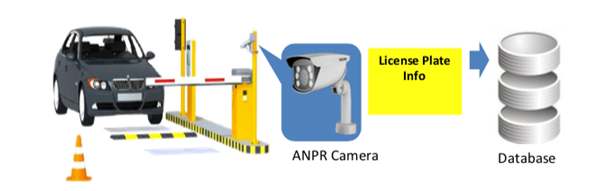
\includegraphics[width=0.8\textwidth]{pics/Taurus_Umsetzung.png}
    \caption{Umsetzung von der Firma Taurus}
    \cite{TaurusUmsetzung}
  \end{figure}
  \newpage
  \section{APERTA [DH]}
  APERTA soll kostengünstig und einfach zu montieren sein. Jedes bereits vorhandene Garagentor kann damit erweitert werden können. Somit fallen keine Kosten für ein neues Tor an. Die Montage sollte von jedem durchgeführt werden können. Auch die Verwaltung der Kennzeichen und sonstigen Bauteile liegt in der Hand des Endverbrauchers oder der Endverbraucherin. Außerdem kann entschieden werden, welche Funktionen die Erweiterungen bieten soll. Der Kunde oder die Kundin müssen somit nicht das Komplettset kaufen. Wird eine verkleinerte Version gekauft, kann diese ganz einfach durch die verfügbaren Module erweitert werden.

  \begin{figure}[H]
    \centering
    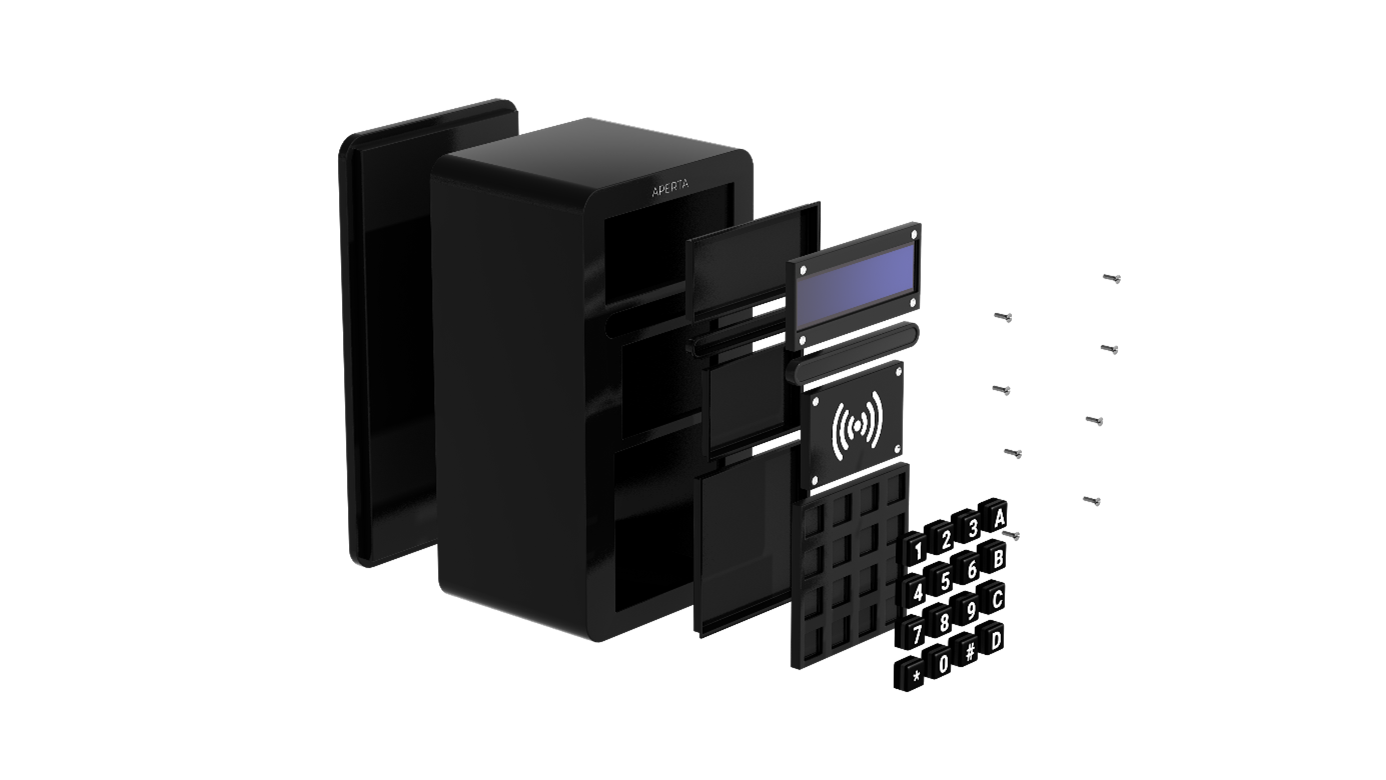
\includegraphics[width=0.8\textwidth]{pics/Modular_Aperta.png}
    \caption{Aperta zerlegt in Module}
  \end{figure}

\begin{spacing}{1}
	\chapter{Persönliche Ziele}\label{chapter:personal Goals}
	\end{spacing}
	\section{Projektverlauf}
\setauthor{David Hauser}

\section{Erkenntnisse von Benjamin Golic}
\setauthor{Benjamin Golic}

\section{Erkenntnisse von David Hauser}
\setauthor{David Hauser}

\section{Erkenntnisse von Simon Koll}
\setauthor{Simon Koll}

Das Projekt nahm immer mehr Substanz an, je weiter die Entwicklung fortschritt. Es kamen neue Ideen hinzu, die Anfangs noch gar nicht im Raum standen. Die Erkenntnisse und Inhalte des ITP-, INSY- sowie SEW-Unterrichts haben mich in der


\begin{spacing}{1}
\chapter{Zusammenfassung / Ausblick}
\end{spacing}
Aufzählungen:

\begin{compactitem}
    \item Itemize Level 1
    \begin{compactitem}
        \item Itemize Level 2
        \begin{compactitem}
            \item Itemize Level 3 (vermeiden)
        \end{compactitem}
    \end{compactitem}
\end{compactitem}

\begin{compactenum}
    \item Enumerate Level 1
    \begin{compactenum}
        \item Enumerate Level 2
        \begin{compactenum}
            \item Enumerate Level 3 (vermeiden)
        \end{compactenum}
    \end{compactenum}
\end{compactenum}

\begin{compactdesc}
    \item[Desc] Level 1
    \begin{compactdesc}
        \item[Desc] Level 2 (vermeiden)
        \begin{compactdesc}
            \item[Desc] Level 3 (vermeiden)
        \end{compactdesc}
    \end{compactdesc}
\end{compactdesc}

\newpage
\pagenumbering{Roman}
\setcounter{page}{\value{RPages}}
\newacronym{guid}{GUID}{Globally Unique Identifier}
\newacronym{jit}{JIT}{Just In Time Compiler}
\newacronym{nfc}{NFC}{Near Field Communication}
\newacronym{rfid}{RFID}{Radio Frequency Identification}

% Usage:
% \gls{label} lowercase in text
% \Gls{label} Uppercase in text
% \newacronym{label}{abbrev}{full}
% \newglossaryentry{label}{settings}



%\setlength{\glsdescwidth}{0.8\linewidth}
\glsnogroupskiptrue
\printglossary[title=Glossar,toctitle=Glossar] %,style=long]
\spacing{1}{
%\bibliographystyle{IEEEtran}
\bibliographystyle{ieeetrande}
\bibliography{bib}
}
\listoffigures
\listoftables
\lstlistoflistings
\appendix
\addchap{Anhang}
\input{./sections/appendix}
\end{document}

